\documentclass[../main.tex]{subfiles}

\begin{document}


%
% -----------------------------------------------------------------------------------------------------------------
%


\begin{frame}[t]{Motivation}

\textbf{Motivation}: Growing interest in multi-functional phased array antennas.

\textbf{Examples}:

\begin{itemize}
    \item Dual-function radar communication (DFRC)
    \item Massive MIMO: 5G technology ($600$MHz - $6$GHz and $24$ - $86$ GHz)
    \item Space-based internet system (Starlink)
\end{itemize}

\textbf{Main reasons}: 
\begin{itemize}
    \item Required spectrum efficiency due to spectrum congestion problem.
    \item Significant reduction in array area, cost and weight.
\end{itemize}


\end{frame}



%
% ----------------------------------------------------------------------------------------------------------------- 
%



\begin{frame}[t]{Digital phased array architecture}

\begin{columns}[t]
    \begin{column}{0.3\textwidth}
    \textbf{Key features}:
    \begin{itemize}
        \item Flexible
        \item Expensive
    \end{itemize}        
    \end{column}
    \begin{column}{0.7\textwidth}
        \begin{figure}[H]
        \begin{adjustbox}{width=0.75\linewidth}
        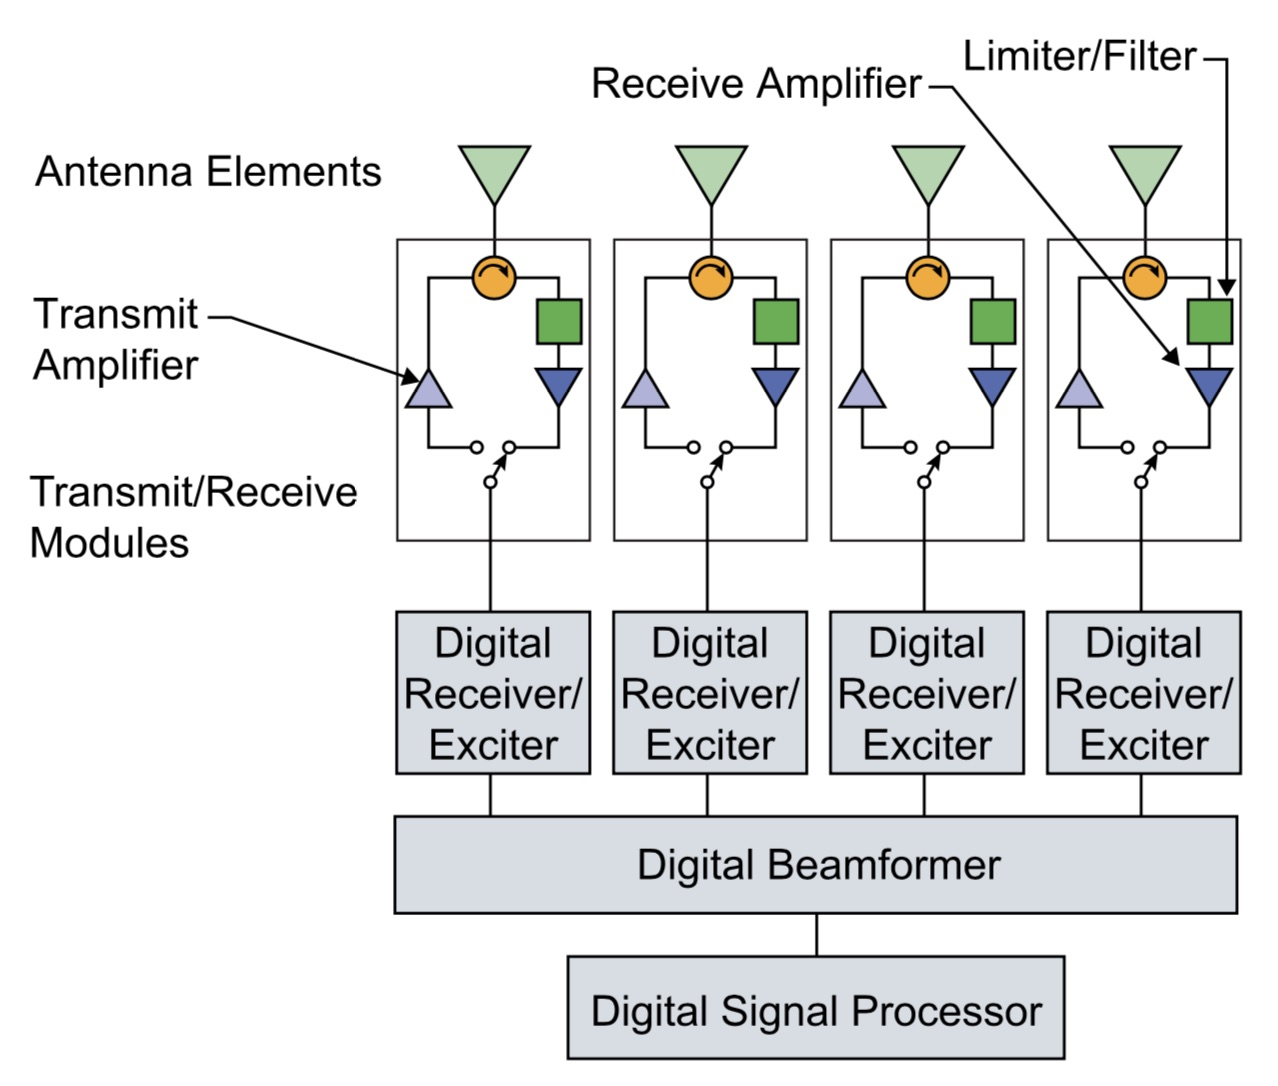
\includegraphics{pics/antenna_structure.jpg}
        \end{adjustbox}
        \end{figure}
    \end{column}
\end{columns}

\end{frame}



%
% ----------------------------------------------------------------------------------------------------------------- 
%



\begin{frame}[t]{Reconfigurable phased antenna arrays. Power amplifier non-linearity}

\textbf{Input}: signals $f_1$ and $f_2$

\textbf{Output}: 
\begin{itemize}
    \item $f_1, f_2$
    \item $2$nd harmonics ($2f_1, 2f_2$) and distortion products ($f_2 \pm f_1$)
    \item $3$rd order distortion ($2f_1 \pm f_2$, $2f_2 \pm f_1$)
\end{itemize}

\begin{figure}[H]
\begin{adjustbox}{width=0.65\linewidth}
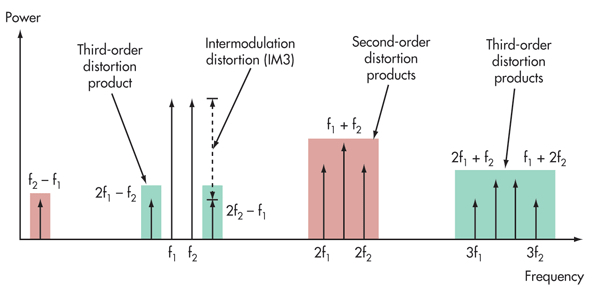
\includegraphics{pics/IMD.jpg}
\end{adjustbox}
\end{figure}


\end{frame}


%
% -----------------------------------------------------------------------------------------------------------------
%

\begin{frame}[t]{Multi-frequency antenna elements allocation}

\begin{figure}[H]
  \centering
  \begin{tikzpicture}
    \draw[thin, color=gray!50] (0, 0) -- (0, 0.5);
    \draw[thin, color=gray!50] (1, 0) -- (1, 0.5);
    \draw[thin, latex'-latex'] (0, 0.5) -- node[above]{$d$} (1, 0.5);

    \draw[thin, -latex', color=gray] (0, 0) -- (-1, 1);
    \coordinate (a1) at (-1, 0);
    \coordinate (b1) at (0, 0);
    \coordinate (c1) at (-1, 1);
    \pic["$\phi_{m}$", draw,<-,>=stealth,angle eccentricity=1.7, angle radius=0.5cm] {angle=c1--b1--a1};
    \draw[thin] (a1) -- (b1);
    \draw[fill] (0,0) circle [radius=0.1] node[below left]{\scriptsize $1$};
    \draw[thin, -latex'] (0, -1) node[below]{$I^{\lambda_k}_1$} -- (0, -0.1);

    \draw[fill] (1,0) circle [radius=0.1] node[below left]{\scriptsize $2$};
    \draw[thin, -latex'] (1, -1) node[below]{$I^{\lambda_k}_2$} -- (1, -0.1);

    \draw[thin, -latex', color=gray] (2, 0) -- (1, 1);
    \draw[fill] (2,0) circle [radius=0.1] node[below left]{\scriptsize $3$};
    \draw[thin, -latex'] (2, -1) node[below]{$I^{\lambda_k}_3$} -- (2, -0.1);

    \draw[draw=black, dotted] (-0.4, -1) rectangle node[below=0.5cm]{$I^{\lambda_k}$} (2.4, -1.7);

    \draw[thin, -latex', color=gray] (3, 0) -- (2, 1);
    \draw[fill] (3,0) circle [radius=0.1] node[below left]{\scriptsize $4$};
    \draw[thin, -latex'] (3, -1) node[below]{$I^{\lambda_{l}}_1$} -- (3, -0.1);

    \draw[dotted, thin](3.5, 0) -- (4.5, 0);

    \draw[thin, -latex', color=gray] (5, 0) -- (4, 1);
    \draw[fill] (5,0) circle [radius=0.1] node[below left]{\scriptsize $N-1$};
    \draw[thin, thin, -latex'] (5, -1) node[below]{$I^{\lambda_{l}}_n$} -- (5, -0.1);
    
    \draw[thin, -latex', color=gray] (6, 0) -- (5, 1);
    \draw[fill] (6,0) circle [radius=0.1] node[below left]{\scriptsize $N$};
    \draw[thin, thin, -latex'] (6, -1) node[below]{$I^{\lambda_{l}}_{n+1}$} -- (6, -0.1);

    \draw[draw=black, dotted] (2.6, -1) rectangle node[below=0.5cm]{$I^{\lambda_l}$} (6.4, -1.7);

  \end{tikzpicture}
\end{figure}

\begin{itemize}
	\item $I^{\lambda_{l}}$ and $I^{\lambda_{k}}$  are randomly allocated currents with wavelengths $\lambda_l$ and $\lambda_k$ for illustration purposes
	\item $\phi_{m}$ is the beam angle, $d$ is the distance between antenna elements
\end{itemize}

\textbf{Assumption}:
Antenna elements are effective radiators in the band of interest (broadband radiators, e.g Vivaldi antennas)

\textbf{Note}:
We aim to allocate one frequency per element

\end{frame}


%
% -----------------------------------------------------------------------------------------------------------------
%

\begin{frame}[t]{Problem formulation}

\textbf{Given:} antenna configuration ($d, N$), reference patterns at different frequencies.

\textbf{Find:} optimal allocation of currents $I^{\lambda_{1\ldots k}}$ among antenna elements
    
\begin{equation*}
\begin{aligned}
& \minimise_{I^{\lambda_{1\ldots k}}} 
& & \Big\| \mathcal{F}^{\lambda_{1 \ldots k}} I^{\lambda_{1\ldots k}} - b^{\lambda_{1 \ldots k}} \Big\|_2^2 \\
& \st
& & I^{\lambda_i} \odot I^{\lambda_j} = 0, \quad \forall i, j \colon i \ne j \\
\end{aligned}
\end{equation*}

where $b^{\lambda_{k}}_m$ is the amplitude of a reference beam with wavelength $\lambda_{k}$ in direction $m$ and
\begin{equation*}
  \mathcal{F}_{\lambda_{1 \ldots k}} = \diag{(\mathcal{F}_{\lambda_1}, \mathcal{F}_{\lambda_2}, \ldots, \mathcal{F}_{\lambda_k})}, \quad \mathcal{F}_{\lambda_{k}} = \Big\{ e^{i \frac{2\pi}{\lambda_k}n d \cos{\phi_m}} \Big\}_{n=0\ldots N, m = 0\ldots M}
\end{equation*}

\textbf{Note}: 
\begin{itemize}
    \item The problem is non-convex, non-linear with a combinatorial constraint, i.e. $k^N$ solutions should be tested ($k$ - number of frequencies, $N$ - number of elements) if unconstrained problem is optimally solvable.
\end{itemize}

\end{frame}


%
% -----------------------------------------------------------------------------------------------------------------
%



\begin{frame}[t]{Objective function choice}

\begin{columns}[t]
\begin{column}{0.5\textwidth}
    Fourier Transform pattern:
    \begin{equation*}
    \minimise_{I^{\lambda_{1\ldots k}}} \Big\| \mathcal{F}^{\lambda_{1 \ldots k}} I^{\lambda_{1\ldots k}} - b^{\lambda_{1 \ldots k}} \Big\|_2^2
    \end{equation*}

    % \begin{equation*}
    % \begin{aligned}
    % & \minimise_{I^{\lambda_{1\ldots k}}} 
    % & & \Big\| \mathcal{F}^{\lambda_{1 \ldots k}} I^{\lambda_{1\ldots k}} - b^{\lambda_{1 \ldots k}} \Big\|_2^2 \\
    % & \st
    % & & (I^{\lambda_{1\ldots k}})^T B I^{\lambda_{1\ldots k}} = 0 \\
    % &&& I^{\lambda_{1\ldots k}} \succeq 0 \\
    % \end{aligned}
    % \end{equation*}

\end{column}
\begin{column}{0.5\textwidth}
    Power pattern:
    \begin{equation*}
    \minimise_{I^{\lambda_{1\ldots k}}}  \Big\| |\mathcal{F}^{\lambda_{1 \ldots k}} I^{\lambda_{1\ldots k}}|^2 - b^{\lambda_{1 \ldots k}} \Big\|_2^2
    \end{equation*}
\end{column}
\end{columns}

\begin{equation*}
\begin{aligned}
& \st
& & (I^{\lambda_{1\ldots k}})^T B I^{\lambda_{1\ldots k}} = 0, \quad \text{\textcolor{gray}{($B=\begin{bmatrix} 0 & I \\ I & 0\end{bmatrix}$ for $2$ different currents)}} \\
&&& I^{\lambda_{1\ldots k}} \succeq 0 \\
\end{aligned}
\end{equation*}

% For $2$ different currents: $B = \begin{bmatrix} 0 & I \\ I & 0\end{bmatrix}$.
\begin{columns}[t]
\begin{column}{0.5\textwidth}
    \textbf{Features}:
    \begin{itemize}
        \item Non-trivial lower bound can be obtained from dual problem:
            \begin{equation*}
            \begin{aligned}
            & \min_{x} 
            & & \Big\{\| Ax - b \|_2^2 + \lambda_{min} (A^TA) x^T B x \Big\} \\
            & \st
            & & x \ge 0 \\
            \end{aligned}
            \end{equation*}
    \end{itemize}
    
\end{column}
\begin{column}{0.5\textwidth}
    \textbf{Features}:
    \begin{itemize}
        \item Quasi-convex objective
        \item Exploiting phases (expect better results)
        \item Unconstrained problem optimality condition leads to \textbf{uncertainty principle} 
    \end{itemize}
\end{column}    
\end{columns}


\end{frame}





%
% -----------------------------------------------------------------------------------------------------------------
%

\begin{frame}[t]{Power pattern. Uncertainty principle}

\begin{equation*}
\Big\| |\mathcal{F}^{\lambda_{1 \ldots k}} I^{\lambda_{1\ldots k}}|^2 - b^{\lambda_{1 \ldots k}} \Big\|_2^2 = \sum_{k=1}^K \sum_{m=1}^M \Big\| (I^{\lambda_{k}})^T Q^{\lambda_{k}}_m  I^{\lambda_{k}} - b^{\lambda_{k}}_m \Big\|_2^2
\end{equation*}


 
\begin{itemize}
	\item It can be shown that the gradient of the objective function is non-zero everywhere except the solution if $\mathcal{N}_{+}(Q^{\lambda_{k}}_m) = \varnothing, ~\forall i$, $Q^{\lambda_{k}}_m = \Real{(\overline{f_m^{\lambda_{k}}} \otimes f_m^{\lambda_{k}})}$.
	\item Analysis of $\mathcal{N}_{+}(Q_i)$ leads to the following conditions:
	\begin{equation*}
  \frac{d}{\lambda} \neq \frac{k}{N+1} \sec \phi_m , \quad \frac{d}{\lambda} \neq \frac{1}{2N} (1 + 2k) \sec \phi_m, \quad \forall m \in \mathbb{Z}^{\ge 0}, \forall k \in \mathbb{Z}
  \label{antenna_design_condition}
	\end{equation*}
	\item These conditions can be interpreted as an \textbf{uncertainty principle} for antenna design: 
\end{itemize}

\begin{center}
\begin{tcolorbox}
\textit{The finer the spacial resolution of the beam is the more values of $\frac{d}{\lambda}$ should be avoided in favour of optimality, i.e. $\mathcal{N}_{+}(Q_i) = \varnothing$.}
\end{tcolorbox}
\end{center}

\end{frame}



\begin{frame}[t]{Practical solution}

\begin{itemize}
\item Introduce $J^{\lambda_k}_n = \log{I^{\lambda_k}_n}$ (this implies $I^{\lambda_k}_n > 0$)
\item Combinatorial constraints are converted into simple linear constraints:
    \begin{equation*}
  J^{\lambda_i} + J^{\lambda_j} \le -\epsilon, \quad \forall i, j \colon i \ne j
    \end{equation*}
    where $\epsilon$ is a design parameter. 
\end{itemize}

Optimisation problem:
\begin{equation*}
\begin{aligned}
& \minimise_{J^{\lambda_{1\ldots k}}} 
& & \sum_{k=1}^K \sum_{m=1}^M \Big\| (e^{J^{\lambda_{k}}})^T Q^{\lambda_{k}}_m  e^{J^{\lambda_{k}}} - b^{\lambda_{k}}_m \Big\|_2^2 \\
& \st
& & J^{\lambda_i} + J^{\lambda_j} \le -\epsilon, \quad \forall i, j \colon i \ne j \\
\end{aligned}
\label{general_problem_formulation3}
\end{equation*}

\end{frame}



\begin{frame}[t]{Algorithm}

\begin{equation*}
\begin{aligned}
& \minimise_{J^{\lambda_{1\ldots k}}} 
& & \sum_{k=1}^K \sum_{m=1}^M \Big\| (e^{J^{\lambda_{k}}})^T Q^{\lambda_{k}}_m  e^{J^{\lambda_{k}}} - b^{\lambda_{k}}_m \Big\|_2^2 \\
& \st
& & M J^{\lambda_{1 \ldots k}} \le - \epsilon
\end{aligned}
\label{general_problem_formulation3}
\end{equation*}

\begin{enumerate}[\color{black}(1)]
    \item Solve unconstrained problem, get $J^*$
    \item Choose $\epsilon = \min{J^*}$. Increase by $\delta \epsilon$.
    \item Solve constrained problem. Return to the previous step
\end{enumerate}

\end{frame}



\begin{frame}[t]{Results. Allocation of three frequencies}

\textbf{Antenna characteristics}:
\begin{itemize}
    \item $100$ elements
    \item $\lambda_1$ 
\end{itemize}

\begin{columns}[t]
        \begin{column}{0.55\textwidth}
            \centering
            \begin{adjustbox}{width=1\columnwidth}
            % This file was created by matlab2tikz.
%
%The latest updates can be retrieved from
%  http://www.mathworks.com/matlabcentral/fileexchange/22022-matlab2tikz-matlab2tikz
%where you can also make suggestions and rate matlab2tikz.
%
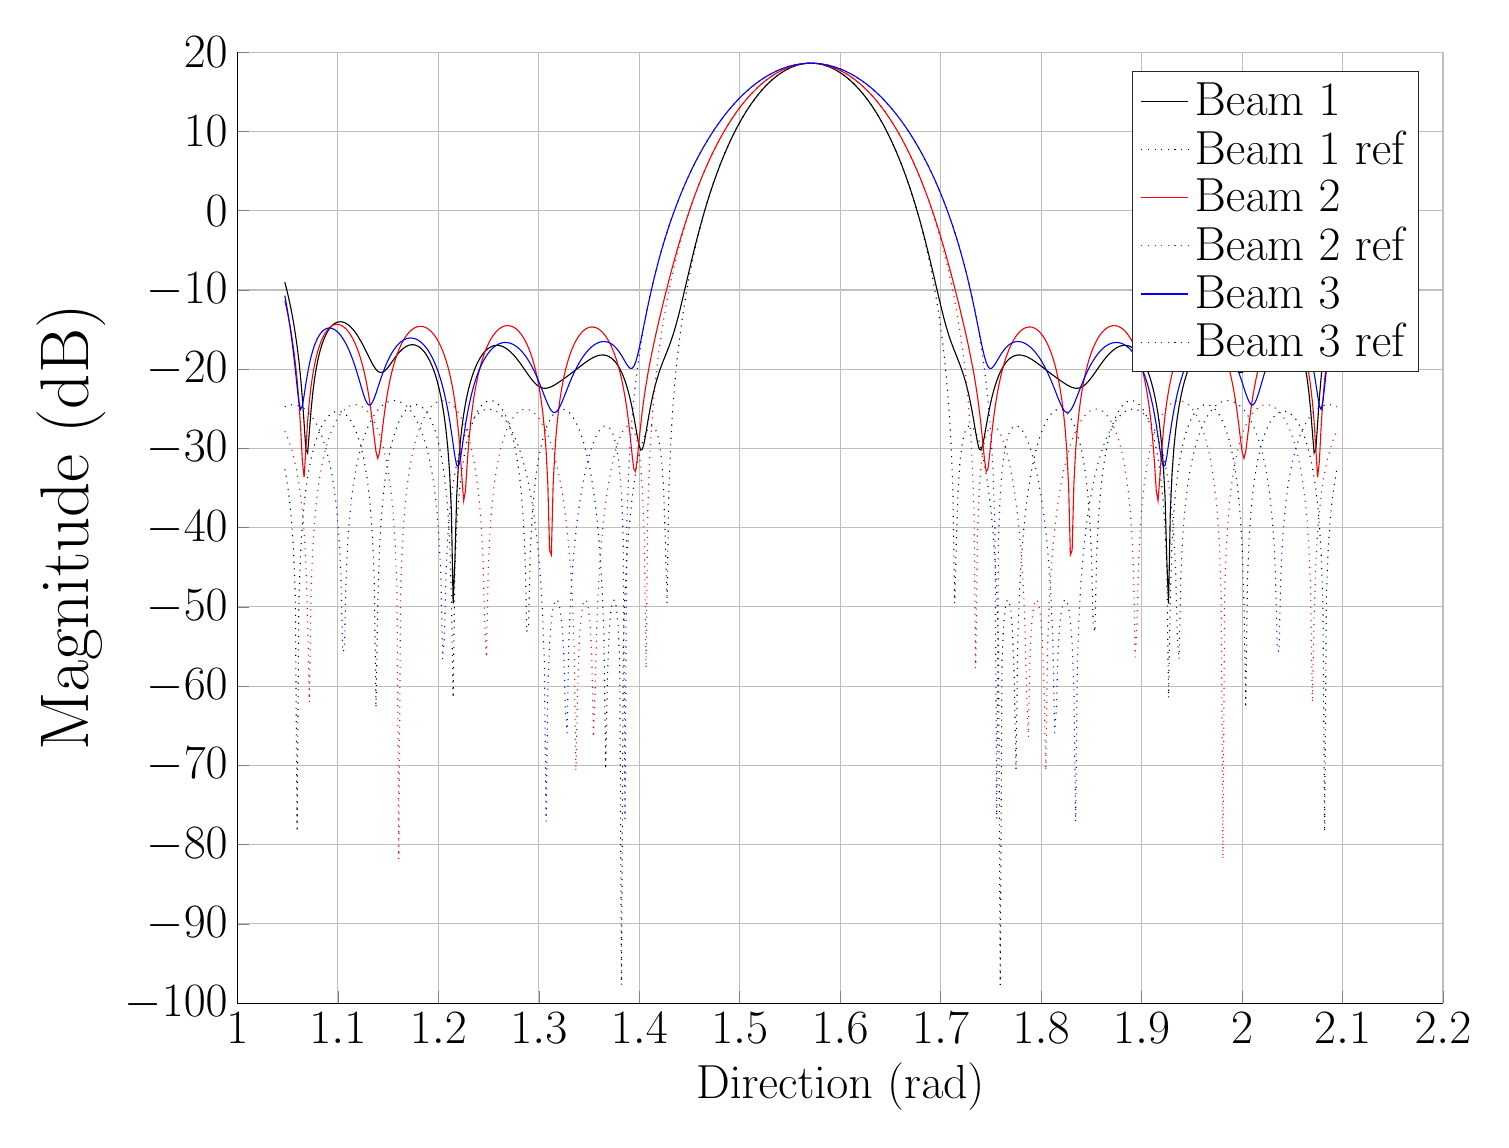
\begin{tikzpicture}

\begin{axis}[%
width=6.028in,
height=4.754in,
at={(1.011in,0.642in)},
scale only axis,
xmin=1,
xmax=2.2,
xlabel={Direction (rad)},
xmajorgrids,
ymin=-100,
ymax=20,
ylabel={Magnitude (dB)},
ymajorgrids,
axis background/.style={fill=white},
axis x line*=bottom,
axis y line*=left,
legend style={legend cell align=left,align=left,draw=white!15!black},
xlabel style={font=\LARGE},ylabel style={font=\Huge},legend style={font=\LARGE},ticklabel style={font=\LARGE}
]
\addplot [color=black,solid]
  table[row sep=crcr]{%
1.0471975511966	-9.00683049941739\\
1.04894288044859	-9.87223771976983\\
1.05068820970059	-10.8053694598435\\
1.05243353895258	-11.818371406769\\
1.05417886820457	-12.9270500696822\\
1.05592419745657	-14.1524853632905\\
1.05766952670856	-15.5235855510198\\
1.05941485596056	-17.0812502750195\\
1.06116018521255	-18.885240372708\\
1.06290551446455	-21.0249191233487\\
1.06465084371654	-23.6295431442648\\
1.06639617296854	-26.8178131001696\\
1.06814150222053	-30.0960076674172\\
1.06988683147252	-30.5712748558198\\
1.07163216072452	-27.8767748540411\\
1.07337748997651	-25.0877892915015\\
1.07512281922851	-22.8835332695111\\
1.0768681484805	-21.1630143956215\\
1.0786134777325	-19.7934486264753\\
1.08035880698449	-18.6818966740696\\
1.08210413623648	-17.7664678082834\\
1.08384946548848	-17.0051596753326\\
1.08559479474047	-16.3685952046567\\
1.08734012399247	-15.835617690836\\
1.08908545324446	-15.3905951827726\\
1.09083078249646	-15.0217255424026\\
1.09257611174845	-14.7199378456408\\
1.09432144100044	-14.4781591650216\\
1.09606677025244	-14.2908118183636\\
1.09781209950443	-14.1534600064623\\
1.09955742875643	-14.0625556572595\\
1.10130275800842	-14.0152514842972\\
1.10304808726042	-14.0092602357899\\
1.10479341651241	-14.0427458485483\\
1.1065387457644	-14.1142363949648\\
1.1082840750164	-14.2225512655996\\
1.11002940426839	-14.3667365023597\\
1.11177473352039	-14.5460028879629\\
1.11352006277238	-14.7596614617971\\
1.11526539202438	-15.0070506361805\\
1.11701072127637	-15.2874480463741\\
1.11875605052837	-15.5999586938275\\
1.12050137978036	-15.9433689163465\\
1.12224670903235	-16.3159535349456\\
1.12399203828435	-16.7152219607235\\
1.12573736753634	-17.1375898271505\\
1.12748269678834	-17.5779692559386\\
1.12922802604033	-18.0292890917289\\
1.13097335529233	-18.4819949405406\\
1.13271868454432	-18.9236461615463\\
1.13446401379631	-19.3388218950549\\
1.13620934304831	-19.7096395888725\\
1.1379546723003	-20.0171932976781\\
1.1397000015523	-20.2440107375586\\
1.14144533080429	-20.3771489942722\\
1.14319066005629	-20.4109850530792\\
1.14493598930828	-20.3485615691472\\
1.14668131856027	-20.2008613335259\\
1.14842664781227	-19.9843538745407\\
1.15017197706426	-19.7178723469686\\
1.15191730631626	-19.4198885496249\\
1.15366263556825	-19.1067503289165\\
1.15540796482025	-18.7919049446203\\
1.15715329407224	-18.4858376298247\\
1.15889862332423	-18.1964057754013\\
1.16064395257623	-17.9293250542555\\
1.16238928182822	-17.68866308383\\
1.16413461108022	-17.4772731764023\\
1.16587994033221	-17.2971474586635\\
1.16762526958421	-17.1496921640415\\
1.1693705988362	-17.0359373076906\\
1.1711159280882	-16.9566950551347\\
1.17286125734019	-16.9126800034085\\
1.17460658659218	-16.9046024729866\\
1.17635191584418	-16.9332437696346\\
1.17809724509617	-16.9995206228905\\
1.17984257434817	-17.1045447676966\\
1.18158790360016	-17.2496829275758\\
1.18333323285216	-17.4366222864601\\
1.18507856210415	-17.6674469426534\\
1.18682389135614	-17.9447319387986\\
1.18856922060814	-18.2716634976335\\
1.19031454986013	-18.6521975142336\\
1.19205987911213	-19.0912739732681\\
1.19380520836412	-19.5951142500327\\
1.19555053761612	-20.1716439660348\\
1.19729586686811	-20.8311115191397\\
1.1990411961201	-21.5870223568938\\
1.2007865253721	-22.4576045417906\\
1.20253185462409	-23.4682148410015\\
1.20427718387609	-24.6555169868149\\
1.20602251312808	-26.07527212966\\
1.20776784238008	-27.8182856173879\\
1.20951317163207	-30.047536753877\\
1.21125850088406	-33.1029096872113\\
1.21300383013606	-37.9111471722467\\
1.21474915938805	-49.5912210303292\\
1.21649448864005	-44.1147399795929\\
1.21823981789204	-36.1348363246076\\
1.21998514714404	-32.0733991612003\\
1.22173047639603	-29.3497875744634\\
1.22347580564802	-27.3139789694257\\
1.22522113490002	-25.7012506346827\\
1.22696646415201	-24.3774215792081\\
1.22871179340401	-23.2650452704823\\
1.230457122656	-22.3153608892781\\
1.232202451908	-21.4956887852964\\
1.23394778115999	-20.7830709231679\\
1.23569311041199	-20.1607759522463\\
1.23743843966398	-19.6162475960306\\
1.23918376891597	-19.1398352489965\\
1.24092909816797	-18.7239739931599\\
1.24267442741996	-18.3626354981809\\
1.24441975667196	-18.0509488465777\\
1.24616508592395	-17.7849316043382\\
1.24791041517595	-17.5612944884296\\
1.24965574442794	-17.3772963626106\\
1.25140107367993	-17.2306343397623\\
1.25314640293193	-17.1193587539242\\
1.25489173218392	-17.0418059313503\\
1.25663706143592	-16.9965437416516\\
1.25838239068791	-16.9823262588794\\
1.26012771993991	-16.9980547552338\\
1.2618730491919	-17.0427428387522\\
1.26361837844389	-17.1154839265793\\
1.26536370769589	-17.2154194796231\\
1.26710903694788	-17.3417065556301\\
1.26885436619988	-17.4934832993817\\
1.27059969545187	-17.6698310120811\\
1.27234502470387	-17.8697314634796\\
1.27409035395586	-18.0920181793064\\
1.27583568320785	-18.3353206250442\\
1.27758101245985	-18.5980006199084\\
1.27932634171184	-18.8780810995157\\
1.28107167096384	-19.1731686957446\\
1.28281700021583	-19.4803737427726\\
1.28456232946783	-19.7962344540719\\
1.28630765871982	-20.1166562131241\\
1.28805298797181	-20.4368818993479\\
1.28979831722381	-20.7515140001458\\
1.2915436464758	-21.0546120613233\\
1.2932889757278	-21.3398869220669\\
1.29503430497979	-21.601002900642\\
1.29677963423179	-21.8319786497274\\
1.29852496348378	-22.0276485907419\\
1.30027029273578	-22.1841172842522\\
1.30201562198777	-22.2991213337117\\
1.30376095123976	-22.372219482138\\
1.30550628049176	-22.404764965813\\
1.30725160974375	-22.3996651729148\\
1.30899693899575	-22.36098280973\\
1.31074226824774	-22.2934617375212\\
1.31248759749974	-22.2020619843278\\
1.31423292675173	-22.0915676902075\\
1.31597825600372	-21.9663015754246\\
1.31772358525572	-21.8299518314752\\
1.31946891450771	-21.6854986327049\\
1.32121424375971	-21.5352186596154\\
1.3229595730117	-21.3807446930464\\
1.3247049022637	-21.2231601747061\\
1.32645023151569	-21.0631129179065\\
1.32819556076768	-20.9009362412562\\
1.32994089001968	-20.7367689848076\\
1.33168621927167	-20.5706680815643\\
1.33343154852367	-20.4027088512417\\
1.33517687777566	-20.2330693104634\\
1.33692220702766	-20.0620958614541\\
1.33866753627965	-19.8903489129233\\
1.34041286553164	-19.7186283359638\\
1.34215819478364	-19.5479800679046\\
1.34390352403563	-19.3796864736115\\
1.34564885328763	-19.2152440717506\\
1.34739418253962	-19.0563327989994\\
1.34913951179162	-18.9047810721147\\
1.35088484104361	-18.7625305633206\\
1.35263017029561	-18.6316039463012\\
1.3543754995476	-18.5140780487621\\
1.35612082879959	-18.4120640093252\\
1.35786615805159	-18.3276952963639\\
1.35961148730358	-18.2631238763217\\
1.36135681655558	-18.2205244493381\\
1.36310214580757	-18.2021064990254\\
1.36484747505957	-18.2101339102783\\
1.36659280431156	-18.2469520661849\\
1.36833813356355	-18.3150226164152\\
1.37008346281555	-18.4169664957382\\
1.37182879206754	-18.5556162514651\\
1.37357412131954	-18.7340793061783\\
1.37531945057153	-18.9558144246263\\
1.37706477982353	-19.2247243279108\\
1.37881010907552	-19.5452679730958\\
1.38055543832751	-19.9225961424657\\
1.38230076757951	-20.3627127885939\\
1.3840460968315	-20.8726599276361\\
1.3857914260835	-21.4607105994565\\
1.38753675533549	-22.1365199116767\\
1.38928208458749	-22.9110972503706\\
1.39102741383948	-23.7962451789529\\
1.39277274309147	-24.8025668865485\\
1.39451807234347	-25.9338095689256\\
1.39626340159546	-27.1722969823029\\
1.39800873084746	-28.445351788001\\
1.39975406009945	-29.5664194938199\\
1.40149938935145	-30.2062272350198\\
1.40324471860344	-30.0694903368892\\
1.40499004785544	-29.2101597544185\\
1.40673537710743	-27.965344455572\\
1.40848070635942	-26.6320629551332\\
1.41022603561142	-25.360416377346\\
1.41197136486341	-24.203209570659\\
1.41371669411541	-23.1690860747524\\
1.4154620233674	-22.2497583268072\\
1.4172073526194	-21.4312600785903\\
1.41895268187139	-20.6980547828971\\
1.42069801112338	-20.0342509998945\\
1.42244334037538	-19.4237237740421\\
1.42418866962737	-18.8499128601692\\
1.42593399887937	-18.2956776455867\\
1.42767932813136	-17.7434462277262\\
1.42942465738336	-17.1758193310519\\
1.43116998663535	-16.5766801254672\\
1.43291531588734	-15.9326774513917\\
1.43466064513934	-15.234730475672\\
1.43640597439133	-14.4790697387986\\
1.43815130364333	-13.6674135153945\\
1.43989663289532	-12.806185197446\\
1.44164196214732	-11.9050393831636\\
1.44338729139931	-10.9751670665273\\
1.4451326206513	-10.0278112058157\\
1.4468779499033	-9.07322972930416\\
1.44862327915529	-8.1201379955419\\
1.45036860840729	-7.17553551305297\\
1.45211393765928	-6.24478185132306\\
1.45385926691128	-5.33180196350433\\
1.45560459616327	-4.43933670282116\\
1.45734992541527	-3.56918887995462\\
1.45909525466726	-2.72244070816725\\
1.46084058391925	-1.89963439070496\\
1.46258591317125	-1.10091621229303\\
1.46433124242324	-0.3261484110161\\
1.46607657167524	0.425005647667697\\
1.46782190092723	1.15301757424161\\
1.46956723017923	1.85844659063782\\
1.47131255943122	2.54190479211287\\
1.47305788868321	3.20403193735205\\
1.47480321793521	3.84547736661866\\
1.4765485471872	4.46688721712459\\
1.4782938764392	5.06889555352424\\
1.48003920569119	5.65211837749488\\
1.48178453494319	6.21714974350977\\
1.48352986419518	6.76455940616729\\
1.48527519344717	7.29489157292863\\
1.48702052269917	7.80866444689744\\
1.48876585195116	8.3063703267448\\
1.49051118120316	8.78847609218193\\
1.49225651045515	9.25542394892309\\
1.49400183970715	9.70763234089078\\
1.49574716895914	10.145496962512\\
1.49749249821113	10.569391822575\\
1.49923782746313	10.979670324921\\
1.50098315671512	11.3766663414632\\
1.50272848596712	11.7606952605864\\
1.50447381521911	12.1320549995408\\
1.50621914447111	12.4910269735331\\
1.5079644737231	12.8378770172015\\
1.5097098029751	13.1728562563146\\
1.51145513222709	13.4962019290851\\
1.51320046147908	13.8081381575752\\
1.51494579073108	14.1088766704229\\
1.51669111998307	14.3986174786188\\
1.51843644923507	14.6775495063789\\
1.52018177848706	14.9458511793391\\
1.52192710773906	15.2036909723819\\
1.52367243699105	15.4512279194169\\
1.52541776624304	15.6886120874014\\
1.52716309549504	15.9159850168155\\
1.52890842474703	16.1334801307147\\
1.53065375399903	16.3412231143731\\
1.53239908325102	16.5393322674168\\
1.53414441250302	16.7279188302286\\
1.53588974175501	16.907087286283\\
1.537635071007	17.0769356419568\\
1.539380400259	17.2375556852448\\
1.54112572951099	17.3890332247008\\
1.54287105876299	17.5314483098208\\
1.54461638801498	17.6648754339859\\
1.54636171726698	17.7893837209885\\
1.54810704651897	17.905037096078\\
1.54985237577096	18.0118944423783\\
1.55159770502296	18.1100097434542\\
1.55334303427495	18.1994322127259\\
1.55508836352695	18.2802064103662\\
1.55683369277894	18.3523723482483\\
1.55857902203094	18.4159655834507\\
1.56032435128293	18.4710173007681\\
1.56206968053493	18.5175543846223\\
1.56381500978692	18.5555994807146\\
1.56556033903891	18.5851710477115\\
1.56730566829091	18.6062833992069\\
1.5690509975429	18.6189467361572\\
1.5707963267949	18.6231671699418\\
1.57254165604689	18.6189467361572\\
1.57428698529889	18.6062833992069\\
1.57603231455088	18.5851710477115\\
1.57777764380287	18.5555994807146\\
1.57952297305487	18.5175543846223\\
1.58126830230686	18.4710173007681\\
1.58301363155886	18.4159655834507\\
1.58475896081085	18.3523723482483\\
1.58650429006285	18.2802064103662\\
1.58824961931484	18.1994322127259\\
1.58999494856683	18.1100097434542\\
1.59174027781883	18.0118944423783\\
1.59348560707082	17.905037096078\\
1.59523093632282	17.7893837209886\\
1.59697626557481	17.6648754339859\\
1.59872159482681	17.5314483098208\\
1.6004669240788	17.3890332247008\\
1.60221225333079	17.2375556852448\\
1.60395758258279	17.0769356419568\\
1.60570291183478	16.907087286283\\
1.60744824108678	16.7279188302286\\
1.60919357033877	16.5393322674168\\
1.61093889959077	16.3412231143731\\
1.61268422884276	16.1334801307147\\
1.61442955809475	15.9159850168155\\
1.61617488734675	15.6886120874014\\
1.61792021659874	15.4512279194169\\
1.61966554585074	15.2036909723819\\
1.62141087510273	14.9458511793391\\
1.62315620435473	14.6775495063789\\
1.62490153360672	14.3986174786189\\
1.62664686285872	14.1088766704229\\
1.62839219211071	13.8081381575752\\
1.6301375213627	13.4962019290851\\
1.6318828506147	13.1728562563146\\
1.63362817986669	12.8378770172015\\
1.63537350911869	12.4910269735331\\
1.63711883837068	12.1320549995409\\
1.63886416762268	11.7606952605864\\
1.64060949687467	11.3766663414632\\
1.64235482612666	10.979670324921\\
1.64410015537866	10.5693918225751\\
1.64584548463065	10.1454969625121\\
1.64759081388265	9.70763234089081\\
1.64933614313464	9.25542394892313\\
1.65108147238664	8.78847609218196\\
1.65282680163863	8.30637032674484\\
1.65457213089062	7.80866444689753\\
1.65631746014262	7.29489157292867\\
1.65806278939461	6.76455940616733\\
1.65980811864661	6.21714974350982\\
1.6615534478986	5.65211837749499\\
1.6632987771506	5.06889555352435\\
1.66504410640259	4.46688721712463\\
1.66678943565458	3.84547736661871\\
1.66853476490658	3.2040319373521\\
1.67028009415857	2.54190479211283\\
1.67202542341057	1.85844659063795\\
1.67377075266256	1.15301757424167\\
1.67551608191456	0.425005647667758\\
1.67726141116655	-0.32614841101604\\
1.67900674041855	-1.10091621229307\\
1.68075206967054	-1.899634390705\\
1.68249739892253	-2.72244070816719\\
1.68424272817453	-3.56918887995455\\
1.68598805742652	-4.43933670282109\\
1.68773338667852	-5.3318019635043\\
1.68947871593051	-6.24478185132312\\
1.69122404518251	-7.1755355130529\\
1.6929693744345	-8.12013799554182\\
1.69471470368649	-9.07322972930409\\
1.69646003293849	-10.0278112058156\\
1.69820536219048	-10.9751670665273\\
1.69995069144248	-11.9050393831634\\
1.70169602069447	-12.8061851974458\\
1.70344134994647	-13.6674135153943\\
1.70518667919846	-14.4790697387986\\
1.70693200845045	-15.2347304756719\\
1.70867733770245	-15.9326774513916\\
1.71042266695444	-16.5766801254671\\
1.71216799620644	-17.1758193310518\\
1.71391332545843	-17.7434462277261\\
1.71565865471043	-18.2956776455867\\
1.71740398396242	-18.8499128601693\\
1.71914931321441	-19.4237237740421\\
1.72089464246641	-20.0342509998942\\
1.7226399717184	-20.6980547828971\\
1.7243853009704	-21.4312600785902\\
1.72613063022239	-22.249758326807\\
1.72787595947439	-23.1690860747527\\
1.72962128872638	-24.2032095706589\\
1.73136661797837	-25.3604163773458\\
1.73311194723037	-26.6320629551331\\
1.73485727648236	-27.9653444555721\\
1.73660260573436	-29.2101597544188\\
1.73834793498635	-30.0694903368888\\
1.74009326423835	-30.2062272350198\\
1.74183859349034	-29.5664194938204\\
1.74358392274234	-28.4453517880011\\
1.74532925199433	-27.1722969823028\\
1.74707458124632	-25.9338095689258\\
1.74881991049832	-24.8025668865485\\
1.75056523975031	-23.796245178953\\
1.75231056900231	-22.9110972503706\\
1.7540558982543	-22.1365199116766\\
1.7558012275063	-21.4607105994567\\
1.75754655675829	-20.8726599276361\\
1.75929188601028	-20.3627127885942\\
1.76103721526228	-19.9225961424658\\
1.76278254451427	-19.545267973096\\
1.76452787376627	-19.2247243279108\\
1.76627320301826	-18.9558144246262\\
1.76801853227026	-18.7340793061782\\
1.76976386152225	-18.5556162514651\\
1.77150919077424	-18.416966495738\\
1.77325452002624	-18.3150226164152\\
1.77499984927823	-18.2469520661849\\
1.77674517853023	-18.2101339102783\\
1.77849050778222	-18.2021064990253\\
1.78023583703422	-18.2205244493382\\
1.78198116628621	-18.2631238763218\\
1.7837264955382	-18.3276952963639\\
1.7854718247902	-18.4120640093252\\
1.78721715404219	-18.5140780487621\\
1.78896248329419	-18.6316039463011\\
1.79070781254618	-18.7625305633207\\
1.79245314179818	-18.9047810721146\\
1.79419847105017	-19.0563327989992\\
1.79594380030217	-19.2152440717504\\
1.79768912955416	-19.3796864736115\\
1.79943445880615	-19.5479800679045\\
1.80117978805815	-19.7186283359637\\
1.80292511731014	-19.8903489129234\\
1.80467044656214	-20.0620958614542\\
1.80641577581413	-20.2330693104634\\
1.80816110506613	-20.4027088512417\\
1.80990643431812	-20.5706680815642\\
1.81165176357011	-20.7367689848073\\
1.81339709282211	-20.9009362412563\\
1.8151424220741	-21.0631129179069\\
1.8168877513261	-21.2231601747063\\
1.81863308057809	-21.3807446930462\\
1.82037840983009	-21.5352186596155\\
1.82212373908208	-21.6854986327048\\
1.82386906833407	-21.8299518314749\\
1.82561439758607	-21.966301575425\\
1.82735972683806	-22.0915676902074\\
1.82910505609006	-22.2020619843277\\
1.83085038534205	-22.293461737521\\
1.83259571459405	-22.3609828097299\\
1.83434104384604	-22.3996651729148\\
1.83608637309803	-22.4047649658132\\
1.83783170235003	-22.3722194821377\\
1.83957703160202	-22.2991213337117\\
1.84132236085402	-22.1841172842523\\
1.84306769010601	-22.0276485907419\\
1.84481301935801	-21.8319786497276\\
1.84655834861	-21.6010029006418\\
1.848303677862	-21.3398869220667\\
1.85004900711399	-21.0546120613231\\
1.85179433636598	-20.7515140001457\\
1.85353966561798	-20.4368818993478\\
1.85528499486997	-20.1166562131243\\
1.85703032412197	-19.7962344540718\\
1.85877565337396	-19.4803737427727\\
1.86052098262596	-19.1731686957446\\
1.86226631187795	-18.8780810995155\\
1.86401164112994	-18.5980006199087\\
1.86575697038194	-18.3353206250444\\
1.86750229963393	-18.0920181793062\\
1.86924762888593	-17.8697314634796\\
1.87099295813792	-17.6698310120808\\
1.87273828738992	-17.4934832993816\\
1.87448361664191	-17.3417065556303\\
1.8762289458939	-17.2154194796233\\
1.8779742751459	-17.1154839265794\\
1.87971960439789	-17.0427428387523\\
1.88146493364989	-16.9980547552336\\
1.88321026290188	-16.9823262588795\\
1.88495559215388	-16.9965437416518\\
1.88670092140587	-17.0418059313502\\
1.88844625065786	-17.1193587539241\\
1.89019157990986	-17.2306343397625\\
1.89193690916185	-17.3772963626104\\
1.89368223841385	-17.5612944884297\\
1.89542756766584	-17.7849316043381\\
1.89717289691784	-18.0509488465777\\
1.89891822616983	-18.3626354981808\\
1.90066355542182	-18.7239739931599\\
1.90240888467382	-19.1398352489964\\
1.90415421392581	-19.6162475960301\\
1.90589954317781	-20.1607759522463\\
1.9076448724298	-20.7830709231678\\
1.9093902016818	-21.4956887852965\\
1.91113553093379	-22.3153608892782\\
1.91288086018578	-23.265045270482\\
1.91462618943778	-24.3774215792081\\
1.91637151868977	-25.7012506346829\\
1.91811684794177	-27.3139789694262\\
1.91986217719376	-29.3497875744633\\
1.92160750644576	-32.0733991611988\\
1.92335283569775	-36.1348363246076\\
1.92509816494975	-44.1147399795961\\
1.92684349420174	-49.5912210303243\\
1.92858882345373	-37.911147172246\\
1.93033415270573	-33.102909687211\\
1.93207948195772	-30.0475367538777\\
1.93382481120972	-27.8182856173885\\
1.93557014046171	-26.0752721296598\\
1.93731546971371	-24.6555169868145\\
1.9390607989657	-23.4682148410008\\
1.94080612821769	-22.4576045417901\\
1.94255145746969	-21.5870223568945\\
1.94429678672168	-20.8311115191394\\
1.94604211597368	-20.1716439660347\\
1.94778744522567	-19.5951142500325\\
1.94953277447767	-19.0912739732679\\
1.95127810372966	-18.6521975142338\\
1.95302343298165	-18.2716634976333\\
1.95476876223365	-17.9447319387988\\
1.95651409148564	-17.6674469426534\\
1.95825942073764	-17.43662228646\\
1.96000474998963	-17.2496829275756\\
1.96175007924163	-17.1045447676967\\
1.96349540849362	-16.9995206228904\\
1.96524073774561	-16.9332437696344\\
1.96698606699761	-16.9046024729862\\
1.9687313962496	-16.9126800034088\\
1.9704767255016	-16.9566950551348\\
1.97222205475359	-17.0359373076904\\
1.97396738400559	-17.1496921640419\\
1.97571271325758	-17.2971474586635\\
1.97745804250958	-17.4772731764022\\
1.97920337176157	-17.6886630838298\\
1.98094870101356	-17.9293250542557\\
1.98269403026556	-18.196405775401\\
1.98443935951755	-18.4858376298251\\
1.98618468876955	-18.7919049446205\\
1.98793001802154	-19.1067503289163\\
1.98967534727354	-19.4198885496245\\
1.99142067652553	-19.7178723469685\\
1.99316600577752	-19.9843538745412\\
1.99491133502952	-20.200861333526\\
1.99665666428151	-20.3485615691471\\
1.99840199353351	-20.410985053079\\
2.0001473227855	-20.3771489942722\\
2.0018926520375	-20.2440107375587\\
2.00363798128949	-20.0171932976781\\
2.00538331054148	-19.7096395888726\\
2.00712863979348	-19.3388218950546\\
2.00887396904547	-18.9236461615461\\
2.01061929829747	-18.4819949405407\\
2.01236462754946	-18.029289091729\\
2.01410995680146	-17.5779692559384\\
2.01585528605345	-17.1375898271507\\
2.01760061530544	-16.7152219607236\\
2.01934594455744	-16.3159535349457\\
2.02109127380943	-15.9433689163466\\
2.02283660306143	-15.5999586938275\\
2.02458193231342	-15.2874480463743\\
2.02632726156542	-15.0070506361805\\
2.02807259081741	-14.759661461797\\
2.02981792006941	-14.5460028879627\\
2.0315632493214	-14.3667365023598\\
2.03330857857339	-14.2225512655996\\
2.03505390782539	-14.114236394965\\
2.03679923707738	-14.0427458485482\\
2.03854456632938	-14.0092602357899\\
2.04028989558137	-14.0152514842973\\
2.04203522483337	-14.0625556572596\\
2.04378055408536	-14.1534600064623\\
2.04552588333735	-14.2908118183634\\
2.04727121258935	-14.4781591650215\\
2.04901654184134	-14.7199378456407\\
2.05076187109334	-15.0217255424027\\
2.05250720034533	-15.3905951827727\\
2.05425252959733	-15.8356176908359\\
2.05599785884932	-16.3685952046567\\
2.05774318810131	-17.0051596753325\\
2.05948851735331	-17.7664678082831\\
2.0612338466053	-18.6818966740699\\
2.0629791758573	-19.7934486264749\\
2.06472450510929	-21.1630143956214\\
2.06646983436129	-22.8835332695114\\
2.06821516361328	-25.087789291501\\
2.06996049286527	-27.8767748540404\\
2.07170582211727	-30.5712748558196\\
2.07345115136926	-30.0960076674157\\
2.07519648062126	-26.817813100169\\
2.07694180987325	-23.6295431442655\\
2.07868713912525	-21.0249191233489\\
2.08043246837724	-18.8852403727078\\
2.08217779762924	-17.0812502750192\\
2.08392312688123	-15.5235855510199\\
2.08566845613322	-14.1524853632907\\
2.08741378538522	-12.9270500696823\\
2.08915911463721	-11.818371406769\\
2.09090444388921	-10.8053694598437\\
2.0926497731412	-9.87223771976988\\
2.0943951023932	-9.00683049941753\\
};
\addlegendentry{Beam 1};

\addplot [color=black,dotted]
  table[row sep=crcr]{%
1.0471975511966	-32.6218102498337\\
1.04894288044859	-33.842384547558\\
1.05068820970059	-35.3185105467661\\
1.05243353895258	-37.1578776046581\\
1.05417886820457	-39.5615358665276\\
1.05592419745657	-42.9773710568606\\
1.05766952670856	-48.809342246416\\
1.05941485596056	-78.3855045333145\\
1.06116018521255	-49.3568945033507\\
1.06290551446455	-43.1804036472629\\
1.06465084371654	-39.6185457216348\\
1.06639617296854	-37.1186542306974\\
1.06814150222053	-35.2031877619444\\
1.06988683147252	-33.6612683485654\\
1.07163216072452	-32.3810446227168\\
1.07337748997651	-31.2960677229696\\
1.07512281922851	-30.3636833239472\\
1.0768681484805	-29.5549312560313\\
1.0786134777325	-28.8493025436441\\
1.08035880698449	-28.2317960953457\\
1.08210413623648	-27.6911627801379\\
1.08384946548848	-27.21880591446\\
1.08559479474047	-26.8080653263583\\
1.08734012399247	-26.4537362009526\\
1.08908545324446	-26.151737478268\\
1.09083078249646	-25.8988789583626\\
1.09257611174845	-25.6926957501314\\
1.09432144100044	-25.5313302020363\\
1.09606677025244	-25.4134485100254\\
1.09781209950443	-25.338183700317\\
1.09955742875643	-25.3050996887163\\
1.10130275800842	-25.3141732424566\\
1.10304808726042	-25.3657923003636\\
1.10479341651241	-25.460770506076\\
1.1065387457644	-25.6003791865286\\
1.1082840750164	-25.7863995685439\\
1.11002940426839	-26.0212000173118\\
1.11177473352039	-26.3078458534243\\
1.11352006277238	-26.650253415468\\
1.11526539202438	-27.0534064203539\\
1.11701072127637	-27.523662995344\\
1.11875605052837	-28.0691990919887\\
1.12050137978036	-28.7006643091949\\
1.12224670903235	-29.4321816137327\\
1.12399203828435	-30.2829293353579\\
1.12573736753634	-31.2797629732828\\
1.12748269678834	-32.4618188506932\\
1.12922802604033	-33.8892185068734\\
1.13097335529233	-35.661222142732\\
1.13271868454432	-37.9596426224691\\
1.13446401379631	-41.17663205619\\
1.13620934304831	-46.4585169218398\\
1.1379546723003	-62.7242647638592\\
1.1397000015523	-49.5852051497503\\
1.14144533080429	-42.6522348100446\\
1.14319066005629	-38.8590565741778\\
1.14493598930828	-36.2487227381274\\
1.14668131856027	-34.2702481606769\\
1.14842664781227	-32.6891992333842\\
1.15017197706426	-31.3838546825639\\
1.15191730631626	-30.2829121534242\\
1.15366263556825	-29.3410622367246\\
1.15540796482025	-28.527779934744\\
1.15715329407224	-27.8215844269617\\
1.15889862332423	-27.2068498296253\\
1.16064395257623	-26.6719182976049\\
1.16238928182822	-26.2079266774152\\
1.16413461108022	-25.8080471506037\\
1.16587994033221	-25.4669798336036\\
1.16762526958421	-25.180605179469\\
1.1693705988362	-24.9457415615209\\
1.1711159280882	-24.7599745682215\\
1.17286125734019	-24.621536977975\\
1.17460658659218	-24.5292260061442\\
1.17635191584418	-24.4823492981201\\
1.17809724509617	-24.4806944401125\\
1.17984257434817	-24.5245191577677\\
1.18158790360016	-24.6145613098276\\
1.18333323285216	-24.7520695795633\\
1.18507856210415	-24.9388577053235\\
1.18682389135614	-25.1773874933045\\
1.18856922060814	-25.4708891595823\\
1.19031454986013	-25.8235324404945\\
1.19205987911213	-26.2406695523506\\
1.19380520836412	-26.7291835532223\\
1.19555053761612	-27.2979968684354\\
1.19729586686811	-27.9588323902344\\
1.1990411961201	-28.7273896723403\\
1.2007865253721	-29.625236763796\\
1.20253185462409	-30.6830086093726\\
1.20427718387609	-31.9461657400496\\
1.20602251312808	-33.4862440522508\\
1.20776784238008	-35.4253865862363\\
1.20951317163207	-37.9989677120523\\
1.21125850088406	-41.7608548483855\\
1.21300383013606	-48.6846920823819\\
1.21474915938805	-61.4907077271486\\
1.21649448864005	-45.391939899449\\
1.21823981789204	-40.0916587140138\\
1.21998514714404	-36.8468215433809\\
1.22173047639603	-34.5188947179127\\
1.22347580564802	-32.7175762990883\\
1.22522113490002	-31.2617713527703\\
1.22696646415201	-30.05259849434\\
1.22871179340401	-29.0301881963747\\
1.230457122656	-28.1556036804115\\
1.232202451908	-27.4021678644899\\
1.23394778115999	-26.7508751149037\\
1.23569311041199	-26.1877782403015\\
1.23743843966398	-25.702412400373\\
1.23918376891597	-25.2868000595705\\
1.24092909816797	-24.9347994591632\\
1.24267442741996	-24.6416656260739\\
1.24441975667196	-24.4037482588058\\
1.24616508592395	-24.2182811095529\\
1.24791041517595	-24.0832348403935\\
1.24965574442794	-23.9972157237454\\
1.25140107367993	-23.9593990627984\\
1.25314640293193	-23.9694905010731\\
1.25489173218392	-24.0277114340254\\
1.25663706143592	-24.1348071269376\\
1.25838239068791	-24.2920783020635\\
1.26012771993991	-24.5014392432264\\
1.2618730491919	-24.7655082697967\\
1.26361837844389	-25.087740284967\\
1.26536370769589	-25.4726168357797\\
1.26710903694788	-25.9259181517182\\
1.26885436619988	-26.4551165227661\\
1.27059969545187	-27.0699560293031\\
1.27234502470387	-27.7833298539381\\
1.27409035395586	-28.6126539953739\\
1.27583568320785	-29.5821122939246\\
1.27758101245985	-30.7265277432891\\
1.27932634171184	-32.0985107759611\\
1.28107167096384	-33.7828976247367\\
1.28281700021583	-35.9297358494569\\
1.28456232946783	-38.8446397120106\\
1.28630765871982	-43.324076916287\\
1.28805298797181	-53.1592614668771\\
1.28979831722381	-52.3392104675345\\
1.2915436464758	-43.106800355638\\
1.2932889757278	-38.781607574602\\
1.29503430497979	-35.9573297303956\\
1.29677963423179	-33.8803652386787\\
1.29852496348378	-32.2569135548622\\
1.30027029273578	-30.9415776237319\\
1.30201562198777	-29.8517855889065\\
1.30376095123976	-28.9362103827406\\
1.30550628049176	-28.1608491728919\\
1.30725160974375	-27.5020970911743\\
1.30899693899575	-26.9429821448522\\
1.31074226824774	-26.4709754040971\\
1.31248759749974	-26.0766478601644\\
1.31423292675173	-25.7528108361048\\
1.31597825600372	-25.4939467977373\\
1.31772358525572	-25.2958222053421\\
1.31946891450771	-25.1552188870275\\
1.32121424375971	-25.0697453338939\\
1.3229595730117	-25.0377037824022\\
1.3247049022637	-25.0579976902926\\
1.32645023151569	-25.1300697096312\\
1.32819556076768	-25.2538638755905\\
1.32994089001968	-25.4298082454601\\
1.33168621927167	-25.6588161165431\\
1.33343154852367	-25.9423055414052\\
1.33517687777566	-26.2822383870381\\
1.33692220702766	-26.6811818773235\\
1.33866753627965	-27.1423976789064\\
1.34041286553164	-27.6699665042249\\
1.34215819478364	-28.2689604802814\\
1.34390352403563	-28.9456821189944\\
1.34564885328763	-29.7079993014948\\
1.34739418253962	-30.565823348353\\
1.34913951179162	-31.5318079675144\\
1.35088484104361	-32.62240280237\\
1.35263017029561	-33.8595026327689\\
1.3543754995476	-35.2731524941665\\
1.35612082879959	-36.9062519041469\\
1.35786615805159	-38.8233706711195\\
1.35961148730358	-41.128987701178\\
1.36135681655558	-44.010795948291\\
1.36310214580757	-47.8663063297995\\
1.36484747505957	-53.8373136057531\\
1.36659280431156	-70.494445956721\\
1.36833813356355	-58.8933595925633\\
1.37008346281555	-52.958068567088\\
1.37182879206754	-50.387949194952\\
1.37357412131954	-49.2563031225635\\
1.37531945057153	-49.1158103355151\\
1.37706477982353	-49.9352912077452\\
1.37881010907552	-52.0515572214253\\
1.38055543832751	-56.8515726032969\\
1.38230076757951	-97.7194545345852\\
1.3840460968315	-55.0807716610022\\
1.3857914260835	-48.2475288181276\\
1.38753675533549	-44.0338273601378\\
1.38928208458749	-40.9352982074641\\
1.39102741383948	-38.4779881076719\\
1.39277274309147	-36.4489998777134\\
1.39451807234347	-34.7339716496171\\
1.39626340159546	-33.2645401948823\\
1.39800873084746	-31.9970161823499\\
1.39975406009945	-30.9023848684229\\
1.40149938935145	-29.9611463198707\\
1.40324471860344	-29.1604963208851\\
1.40499004785544	-28.4927709826471\\
1.40673537710743	-27.9546623822378\\
1.40848070635942	-27.5469896285109\\
1.41022603561142	-27.2749723396476\\
1.41197136486341	-27.1490908498114\\
1.41371669411541	-27.1867982985077\\
1.4154620233674	-27.4156793018878\\
1.4172073526194	-27.8793744555672\\
1.41895268187139	-28.6494189404466\\
1.42069801112338	-29.8514986673935\\
1.42244334037538	-31.7337335424752\\
1.42418866962737	-34.8970061378204\\
1.42593399887937	-41.6168863744207\\
1.42767932813136	-49.5492682808495\\
1.42942465738336	-35.3631333801778\\
1.43116998663535	-29.6232501285043\\
1.43291531588734	-25.7815421974949\\
1.43466064513934	-22.8146764965761\\
1.43640597439133	-20.3584929407565\\
1.43815130364333	-18.2405371823621\\
1.43989663289532	-16.365200010593\\
1.44164196214732	-14.6737916769396\\
1.44338729139931	-13.1276019087821\\
1.4451326206513	-11.6996919421882\\
1.4468779499033	-10.370517594109\\
1.44862327915529	-9.12541894127639\\
1.45036860840729	-7.953095473714\\
1.45211393765928	-6.8446357265022\\
1.45385926691128	-5.79287549350553\\
1.45560459616327	-4.79195933960004\\
1.45734992541527	-3.83703257045766\\
1.45909525466726	-2.92401957872692\\
1.46084058391925	-2.04946095485101\\
1.46258591317125	-1.21039154060547\\
1.46433124242324	-0.404247615298435\\
1.46607657167524	0.371204796297414\\
1.46782190092723	1.11792604255476\\
1.46956723017923	1.83764730536604\\
1.47131255943122	2.53190621221738\\
1.47305788868321	3.20207564783365\\
1.47480321793521	3.84938727892531\\
1.4765485471872	4.47495092510673\\
1.4782938764392	5.0797706342991\\
1.48003920569119	5.66475811992941\\
1.48178453494319	6.23074406841036\\
1.48352986419518	6.77848771395871\\
1.48527519344717	7.30868499352271\\
1.48702052269917	7.82197553020474\\
1.48876585195116	8.31894864395113\\
1.49051118120316	8.80014854971174\\
1.49225651045515	9.26607887306369\\
1.49400183970715	9.71720658944589\\
1.49574716895914	10.1539654741991\\
1.49749249821113	10.5767591354421\\
1.49923782746313	10.9859636896068\\
1.50098315671512	11.3819301295641\\
1.50272848596712	11.7649864272213\\
1.50447381521911	12.1354394058752\\
1.50621914447111	12.4935764121771\\
1.5079644737231	12.8396668130786\\
1.5097098029751	13.1739633393946\\
1.51145513222709	13.4967032945101\\
1.51320046147908	13.808109644146\\
1.51494579073108	14.108392000907\\
1.51669111998307	14.397747515478\\
1.51843644923507	14.6763616847634\\
1.52018177848706	14.9444090859289\\
1.52192710773906	15.2020540441569\\
1.52367243699105	15.4494512409552\\
1.52541776624304	15.6867462690108\\
1.52716309549504	15.9140761388599\\
1.52890842474703	16.1315697420159\\
1.53065375399903	16.3393482746517\\
1.53239908325102	16.5375256254638\\
1.53414441250302	16.7262087309264\\
1.53588974175501	16.9054979007882\\
1.537635071007	17.0754871163436\\
1.539380400259	17.2362643037329\\
1.54112572951099	17.3879115842794\\
1.54287105876299	17.5305055036542\\
1.54461638801498	17.664117241465\\
1.54636171726698	17.7888128026943\\
1.54810704651897	17.9046531922586\\
1.54985237577096	18.0116945738213\\
1.55159770502296	18.1099884138715\\
1.55334303427495	18.1995816119647\\
1.55508836352695	18.2805166179243\\
1.55683369277894	18.3528315367093\\
1.55857902203094	18.4165602215681\\
1.56032435128293	18.471732356024\\
1.56206968053493	18.5183735251632\\
1.56381500978692	18.5565052766332\\
1.56556033903891	18.5861451716941\\
1.56730566829091	18.6073068266084\\
1.5690509975429	18.6199999445997\\
1.5707963267949	18.6242303385555\\
1.57254165604689	18.6199999445997\\
1.57428698529889	18.6073068266084\\
1.57603231455088	18.5861451716941\\
1.57777764380287	18.5565052766332\\
1.57952297305487	18.5183735251632\\
1.58126830230686	18.471732356024\\
1.58301363155886	18.4165602215681\\
1.58475896081085	18.3528315367093\\
1.58650429006285	18.2805166179243\\
1.58824961931484	18.1995816119647\\
1.58999494856683	18.1099884138715\\
1.59174027781883	18.0116945738213\\
1.59348560707082	17.9046531922586\\
1.59523093632282	17.7888128026943\\
1.59697626557481	17.664117241465\\
1.59872159482681	17.5305055036542\\
1.6004669240788	17.3879115842794\\
1.60221225333079	17.2362643037329\\
1.60395758258279	17.0754871163436\\
1.60570291183478	16.9054979007882\\
1.60744824108678	16.7262087309264\\
1.60919357033877	16.5375256254638\\
1.61093889959077	16.3393482746517\\
1.61268422884276	16.1315697420158\\
1.61442955809475	15.9140761388599\\
1.61617488734675	15.6867462690108\\
1.61792021659874	15.4494512409552\\
1.61966554585074	15.2020540441569\\
1.62141087510273	14.9444090859288\\
1.62315620435473	14.6763616847634\\
1.62490153360672	14.397747515478\\
1.62664686285872	14.1083920009071\\
1.62839219211071	13.808109644146\\
1.6301375213627	13.4967032945101\\
1.6318828506147	13.1739633393946\\
1.63362817986669	12.8396668130786\\
1.63537350911869	12.4935764121771\\
1.63711883837068	12.1354394058753\\
1.63886416762268	11.7649864272213\\
1.64060949687467	11.3819301295641\\
1.64235482612666	10.9859636896068\\
1.64410015537866	10.5767591354421\\
1.64584548463065	10.1539654741992\\
1.64759081388265	9.71720658944593\\
1.64933614313464	9.26607887306373\\
1.65108147238664	8.80014854971178\\
1.65282680163863	8.31894864395117\\
1.65457213089062	7.82197553020483\\
1.65631746014262	7.30868499352275\\
1.65806278939461	6.77848771395876\\
1.65980811864661	6.2307440684104\\
1.6615534478986	5.66475811992952\\
1.6632987771506	5.07977063429922\\
1.66504410640259	4.47495092510677\\
1.66678943565458	3.84938727892535\\
1.66853476490658	3.2020756478337\\
1.67028009415857	2.53190621221733\\
1.67202542341057	1.83764730536618\\
1.67377075266256	1.11792604255482\\
1.67551608191456	0.371204796297468\\
1.67726141116655	-0.404247615298374\\
1.67900674041855	-1.21039154060552\\
1.68075206967054	-2.04946095485105\\
1.68249739892253	-2.92401957872686\\
1.68424272817453	-3.83703257045758\\
1.68598805742652	-4.79195933959999\\
1.68773338667852	-5.79287549350545\\
1.68947871593051	-6.84463572650226\\
1.69122404518251	-7.95309547371392\\
1.6929693744345	-9.12541894127628\\
1.69471470368649	-10.3705175941089\\
1.69646003293849	-11.6996919421881\\
1.69820536219048	-13.127601908782\\
1.69995069144248	-14.6737916769393\\
1.70169602069447	-16.3652000105927\\
1.70344134994647	-18.2405371823617\\
1.70518667919846	-20.3584929407564\\
1.70693200845045	-22.814676496576\\
1.70867733770245	-25.7815421974943\\
1.71042266695444	-29.6232501285034\\
1.71216799620644	-35.3631333801777\\
1.71391332545843	-49.5492682808483\\
1.71565865471043	-41.6168863744217\\
1.71740398396242	-34.8970061378202\\
1.71914931321441	-31.7337335424751\\
1.72089464246641	-29.8514986673938\\
1.7226399717184	-28.6494189404466\\
1.7243853009704	-27.8793744555673\\
1.72613063022239	-27.415679301888\\
1.72787595947439	-27.1867982985078\\
1.72962128872638	-27.1490908498113\\
1.73136661797837	-27.2749723396474\\
1.73311194723037	-27.5469896285109\\
1.73485727648236	-27.9546623822377\\
1.73660260573436	-28.4927709826467\\
1.73834793498635	-29.1604963208853\\
1.74009326423835	-29.9611463198707\\
1.74183859349034	-30.9023848684231\\
1.74358392274234	-31.9970161823496\\
1.74532925199433	-33.2645401948822\\
1.74707458124632	-34.7339716496168\\
1.74881991049832	-36.4489998777132\\
1.75056523975031	-38.477988107671\\
1.75231056900231	-40.9352982074642\\
1.7540558982543	-44.0338273601384\\
1.7558012275063	-48.2475288181273\\
1.75754655675829	-55.0807716610024\\
1.75929188601028	-97.7194545350483\\
1.76103721526228	-56.8515726032971\\
1.76278254451427	-52.0515572214307\\
1.76452787376627	-49.9352912077444\\
1.76627320301826	-49.1158103355151\\
1.76801853227026	-49.2563031225632\\
1.76976386152225	-50.3879491949528\\
1.77150919077424	-52.9580685670892\\
1.77325452002624	-58.8933595925653\\
1.77499984927823	-70.4944459567078\\
1.77674517853023	-53.8373136057519\\
1.77849050778222	-47.8663063298008\\
1.78023583703422	-44.0107959482909\\
1.78198116628621	-41.1289877011784\\
1.7837264955382	-38.8233706711201\\
1.7854718247902	-36.9062519041469\\
1.78721715404219	-35.2731524941667\\
1.78896248329419	-33.8595026327684\\
1.79070781254618	-32.6224028023698\\
1.79245314179818	-31.5318079675143\\
1.79419847105017	-30.5658233483528\\
1.79594380030217	-29.7079993014951\\
1.79768912955416	-28.9456821189945\\
1.79943445880615	-28.2689604802818\\
1.80117978805815	-27.6699665042248\\
1.80292511731014	-27.1423976789067\\
1.80467044656214	-26.6811818773234\\
1.80641577581413	-26.2822383870381\\
1.80816110506613	-25.9423055414051\\
1.80990643431812	-25.658816116543\\
1.81165176357011	-25.4298082454602\\
1.81339709282211	-25.2538638755906\\
1.8151424220741	-25.1300697096311\\
1.8168877513261	-25.0579976902926\\
1.81863308057809	-25.0377037824022\\
1.82037840983009	-25.0697453338937\\
1.82212373908208	-25.1552188870276\\
1.82386906833407	-25.295822205342\\
1.82561439758607	-25.4939467977374\\
1.82735972683806	-25.7528108361048\\
1.82910505609006	-26.0766478601643\\
1.83085038534205	-26.4709754040971\\
1.83259571459405	-26.9429821448522\\
1.83434104384604	-27.5020970911745\\
1.83608637309803	-28.160849172892\\
1.83783170235003	-28.9362103827405\\
1.83957703160202	-29.8517855889063\\
1.84132236085402	-30.941577623732\\
1.84306769010601	-32.2569135548621\\
1.84481301935801	-33.8803652386783\\
1.84655834861	-35.9573297303962\\
1.848303677862	-38.7816075746017\\
1.85004900711399	-43.1068003556391\\
1.85179433636598	-52.3392104675322\\
1.85353966561798	-53.1592614668821\\
1.85528499486997	-43.3240769162895\\
1.85703032412197	-38.8446397120107\\
1.85877565337396	-35.9297358494575\\
1.86052098262596	-33.782897624737\\
1.86226631187795	-32.0985107759611\\
1.86401164112994	-30.726527743289\\
1.86575697038194	-29.582112293925\\
1.86750229963393	-28.6126539953739\\
1.86924762888593	-27.7833298539383\\
1.87099295813792	-27.0699560293029\\
1.87273828738992	-26.455116522766\\
1.87448361664191	-25.9259181517183\\
1.8762289458939	-25.4726168357797\\
1.8779742751459	-25.0877402849671\\
1.87971960439789	-24.7655082697966\\
1.88146493364989	-24.5014392432265\\
1.88321026290188	-24.2920783020635\\
1.88495559215388	-24.1348071269376\\
1.88670092140587	-24.0277114340253\\
1.88844625065786	-23.9694905010732\\
1.89019157990986	-23.9593990627985\\
1.89193690916185	-23.9972157237455\\
1.89368223841385	-24.0832348403934\\
1.89542756766584	-24.2182811095529\\
1.89717289691784	-24.4037482588059\\
1.89891822616983	-24.6416656260737\\
1.90066355542182	-24.9347994591633\\
1.90240888467382	-25.2868000595703\\
1.90415421392581	-25.7024124003726\\
1.90589954317781	-26.1877782403016\\
1.9076448724298	-26.7508751149038\\
1.9093902016818	-27.4021678644901\\
1.91113553093379	-28.1556036804113\\
1.91288086018578	-29.0301881963744\\
1.91462618943778	-30.0525984943399\\
1.91637151868977	-31.2617713527704\\
1.91811684794177	-32.7175762990885\\
1.91986217719376	-34.5188947179122\\
1.92160750644576	-36.8468215433799\\
1.92335283569775	-40.0916587140141\\
1.92509816494975	-45.3919398994491\\
1.92684349420174	-61.4907077271674\\
1.92858882345373	-48.6846920823807\\
1.93033415270573	-41.7608548483839\\
1.93207948195772	-37.9989677120527\\
1.93382481120972	-35.4253865862372\\
1.93557014046171	-33.4862440522508\\
1.93731546971371	-31.9461657400489\\
1.9390607989657	-30.6830086093724\\
1.94080612821769	-29.6252367637962\\
1.94255145746969	-28.7273896723403\\
1.94429678672168	-27.9588323902339\\
1.94604211597368	-27.2979968684353\\
1.94778744522567	-26.7291835532225\\
1.94953277447767	-26.2406695523508\\
1.95127810372966	-25.8235324404948\\
1.95302343298165	-25.4708891595825\\
1.95476876223365	-25.1773874933049\\
1.95651409148564	-24.9388577053234\\
1.95825942073764	-24.7520695795633\\
1.96000474998963	-24.6145613098277\\
1.96175007924163	-24.5245191577676\\
1.96349540849362	-24.4806944401124\\
1.96524073774561	-24.48234929812\\
1.96698606699761	-24.5292260061441\\
1.9687313962496	-24.621536977975\\
1.9704767255016	-24.7599745682215\\
1.97222205475359	-24.9457415615208\\
1.97396738400559	-25.1806051794691\\
1.97571271325758	-25.4669798336034\\
1.97745804250958	-25.8080471506037\\
1.97920337176157	-26.207926677415\\
1.98094870101356	-26.6719182976049\\
1.98269403026556	-27.2068498296254\\
1.98443935951755	-27.8215844269617\\
1.98618468876955	-28.5277799347439\\
1.98793001802154	-29.3410622367243\\
1.98967534727354	-30.2829121534241\\
1.99142067652553	-31.3838546825643\\
1.99316600577752	-32.6891992333844\\
1.99491133502952	-34.2702481606764\\
1.99665666428151	-36.2487227381269\\
1.99840199353351	-38.8590565741765\\
2.0001473227855	-42.6522348100436\\
2.0018926520375	-49.5852051497518\\
2.00363798128949	-62.7242647638484\\
2.00538331054148	-46.4585169218385\\
2.00712863979348	-41.1766320561906\\
2.00887396904547	-37.95964262247\\
2.01061929829747	-35.661222142732\\
2.01236462754946	-33.8892185068738\\
2.01410995680146	-32.4618188506929\\
2.01585528605345	-31.2797629732827\\
2.01760061530544	-30.2829293353581\\
2.01934594455744	-29.4321816137329\\
2.02109127380943	-28.7006643091948\\
2.02283660306143	-28.0691990919892\\
2.02458193231342	-27.5236629953441\\
2.02632726156542	-27.0534064203541\\
2.02807259081741	-26.6502534154676\\
2.02981792006941	-26.3078458534244\\
2.0315632493214	-26.0212000173118\\
2.03330857857339	-25.7863995685441\\
2.03505390782539	-25.6003791865283\\
2.03679923707738	-25.4607705060759\\
2.03854456632938	-25.3657923003636\\
2.04028989558137	-25.3141732424566\\
2.04203522483337	-25.3050996887164\\
2.04378055408536	-25.338183700317\\
2.04552588333735	-25.4134485100256\\
2.04727121258935	-25.5313302020364\\
2.04901654184134	-25.692695750131\\
2.05076187109334	-25.8988789583626\\
2.05250720034533	-26.1517374782679\\
2.05425252959733	-26.4537362009525\\
2.05599785884932	-26.8080653263583\\
2.05774318810131	-27.2188059144603\\
2.05948851735331	-27.6911627801378\\
2.0612338466053	-28.231796095346\\
2.0629791758573	-28.849302543644\\
2.06472450510929	-29.5549312560315\\
2.06646983436129	-30.3636833239472\\
2.06821516361328	-31.29606772297\\
2.06996049286527	-32.3810446227167\\
2.07170582211727	-33.6612683485656\\
2.07345115136926	-35.2031877619449\\
2.07519648062126	-37.1186542306985\\
2.07694180987325	-39.618545721635\\
2.07868713912525	-43.180403647262\\
2.08043246837724	-49.3568945033515\\
2.08217779762924	-78.3855045332927\\
2.08392312688123	-48.8093422464176\\
2.08566845613322	-42.9773710568608\\
2.08741378538522	-39.5615358665269\\
2.08915911463721	-37.1578776046575\\
2.09090444388921	-35.3185105467658\\
2.0926497731412	-33.8423845475579\\
2.0943951023932	-32.621810249834\\
};
\addlegendentry{Beam 1 ref};

\addplot [color=red,solid]
  table[row sep=crcr]{%
1.0471975511966	-11.3572514855639\\
1.04894288044859	-12.3269833125542\\
1.05068820970059	-13.3921083679584\\
1.05243353895258	-14.5733281074036\\
1.05417886820457	-15.8993077320696\\
1.05592419745657	-17.4112439561481\\
1.05766952670856	-19.1710525199192\\
1.05941485596056	-21.2767819199081\\
1.06116018521255	-23.891891263129\\
1.06290551446455	-27.2849723221499\\
1.06465084371654	-31.5940782557831\\
1.06639617296854	-33.6395662123999\\
1.06814150222053	-30.144507844149\\
1.06988683147252	-26.6188665252598\\
1.07163216072452	-24.0341699203141\\
1.07337748997651	-22.0969925683265\\
1.07512281922851	-20.5887546476995\\
1.0768681484805	-19.3801027643554\\
1.0786134777325	-18.3920250223573\\
1.08035880698449	-17.5736442474612\\
1.08210413623648	-16.890610964129\\
1.08384946548848	-16.3188144632706\\
1.08559479474047	-15.8407954508646\\
1.08734012399247	-15.4435975420272\\
1.08908545324446	-15.1174245546052\\
1.09083078249646	-14.8547705334887\\
1.09257611174845	-14.6498389065932\\
1.09432144100044	-14.4981452360786\\
1.09606677025244	-14.3962406466448\\
1.09781209950443	-14.3415172504862\\
1.09955742875643	-14.3320712076898\\
1.10130275800842	-14.3666078394943\\
1.10304808726042	-14.444378808238\\
1.10479341651241	-14.5651451149735\\
1.1065387457644	-14.7291623197676\\
1.1082840750164	-14.9371864439075\\
1.11002940426839	-15.190500796535\\
1.11177473352039	-15.4909657369601\\
1.11352006277238	-15.8410953757375\\
1.11526539202438	-16.2441676927251\\
1.11701072127637	-16.7043778250965\\
1.11875605052837	-17.2270487423783\\
1.12050137978036	-17.8189195983347\\
1.12224670903235	-18.4885399199468\\
1.12399203828435	-19.2468064390263\\
1.12573736753634	-20.1076831990823\\
1.12748269678834	-21.0891230968347\\
1.12922802604033	-22.214083979557\\
1.13097335529233	-23.5110353160907\\
1.13271868454432	-25.0115105417305\\
1.13446401379631	-26.7355614835132\\
1.13620934304831	-28.6332745837722\\
1.1379546723003	-30.4024916252066\\
1.1397000015523	-31.2486839366019\\
1.14144533080429	-30.528142901106\\
1.14319066005629	-28.8190078633365\\
1.14493598930828	-26.9436188251643\\
1.14668131856027	-25.2320940811421\\
1.14842664781227	-23.743609968374\\
1.15017197706426	-22.4600467436584\\
1.15191730631626	-21.3498045990101\\
1.15366263556825	-20.3839087619729\\
1.15540796482025	-19.5388584349748\\
1.15715329407224	-18.7962050895789\\
1.15889862332423	-18.141539008058\\
1.16064395257623	-17.5635517564244\\
1.16238928182822	-17.0532981879323\\
1.16413461108022	-16.603643466014\\
1.16587994033221	-16.2088545705934\\
1.16762526958421	-15.8642987238582\\
1.1693705988362	-15.5662196896101\\
1.1711159280882	-15.3115707937578\\
1.17286125734019	-15.0978895913895\\
1.17460658659218	-14.923203507106\\
1.17635191584418	-14.7859588981819\\
1.17809724509617	-14.6849682025804\\
1.17984257434817	-14.6193714171543\\
1.18158790360016	-14.5886093077837\\
1.18333323285216	-14.5924066258004\\
1.18507856210415	-14.6307642967541\\
1.18682389135614	-14.7039601356744\\
1.18856922060814	-14.812558190729\\
1.19031454986013	-14.9574273831526\\
1.19205987911213	-15.1397707585974\\
1.19380520836412	-15.361167471795\\
1.19555053761612	-15.623630700535\\
1.19729586686811	-15.9296861864536\\
1.1990411961201	-16.2824782784168\\
1.2007865253721	-16.6859136120886\\
1.20253185462409	-17.1448575672003\\
1.20427718387609	-17.6654065510517\\
1.20602251312808	-18.2552719891272\\
1.20776784238008	-18.9243333421888\\
1.20951317163207	-19.6854544039233\\
1.21125850088406	-20.5557228318007\\
1.21300383013606	-21.558393413372\\
1.21474915938805	-22.7260420931713\\
1.21649448864005	-24.1058619311985\\
1.21823981789204	-25.7687407485599\\
1.21998514714404	-27.8241158782265\\
1.22173047639603	-30.4341371152484\\
1.22347580564802	-33.7161835528627\\
1.22522113490002	-36.5976911327758\\
1.22696646415201	-35.3703104645539\\
1.22871179340401	-31.9457658523483\\
1.230457122656	-28.9982142103773\\
1.232202451908	-26.6902521412101\\
1.23394778115999	-24.8473856298548\\
1.23569311041199	-23.3349973276019\\
1.23743843966398	-22.0656810311477\\
1.23918376891597	-20.9821775432699\\
1.24092909816797	-20.0456594389993\\
1.24267442741996	-19.2288505685007\\
1.24441975667196	-18.5119824393414\\
1.24616508592395	-17.8803450047817\\
1.24791041517595	-17.3227502644115\\
1.24965574442794	-16.8305356987246\\
1.25140107367993	-16.3968981233626\\
1.25314640293193	-16.0164365208852\\
1.25489173218392	-15.6848311058293\\
1.25663706143592	-15.3986137119133\\
1.25838239068791	-15.1550010076663\\
1.26012771993991	-14.9517720252574\\
1.2618730491919	-14.787177726988\\
1.26361837844389	-14.659874344416\\
1.26536370769589	-14.5688748757964\\
1.26710903694788	-14.5135149340502\\
1.26885436619988	-14.493430415349\\
1.27059969545187	-14.5085454080679\\
1.27234502470387	-14.5590695173735\\
1.27409035395586	-14.6455044393025\\
1.27583568320785	-14.7686602595186\\
1.27758101245985	-14.9296826529943\\
1.27932634171184	-15.1300930103331\\
1.28107167096384	-15.3718446321729\\
1.28281700021583	-15.6573996881203\\
1.28456232946783	-15.9898339019108\\
1.28630765871982	-16.3729793439179\\
1.28805298797181	-16.8116210409235\\
1.28979831722381	-17.3117716823881\\
1.2915436464758	-17.8810629479467\\
1.2932889757278	-18.5293165464322\\
1.29503430497979	-19.2694022200327\\
1.29677963423179	-20.1185732928736\\
1.29852496348378	-21.1006367963027\\
1.30027029273578	-22.2496713922021\\
1.30201562198777	-23.6168359709047\\
1.30376095123976	-25.2839637917353\\
1.30550628049176	-27.394069847618\\
1.30725160974375	-30.2323305432546\\
1.30899693899575	-34.506144758764\\
1.31074226824774	-42.8662292820693\\
1.31248759749974	-43.4298389061284\\
1.31423292675173	-34.7398723800068\\
1.31597825600372	-30.3717720846543\\
1.31772358525572	-27.4904266791174\\
1.31946891450771	-25.3554622912487\\
1.32121424375971	-23.6721611716114\\
1.3229595730117	-22.2938054160129\\
1.3247049022637	-21.1368618223284\\
1.32645023151569	-20.1493089626814\\
1.32819556076768	-19.2966065426027\\
1.32994089001968	-18.5546980239069\\
1.33168621927167	-17.9062019772702\\
1.33343154852367	-17.3381947072015\\
1.33517687777566	-16.8408485024041\\
1.33692220702766	-16.4065583679673\\
1.33866753627965	-16.0293617483334\\
1.34041286553164	-15.7045414514333\\
1.34215819478364	-15.4283473068442\\
1.34390352403563	-15.1977972544711\\
1.34564885328763	-15.0105331300486\\
1.34739418253962	-14.8647151673397\\
1.34913951179162	-14.7589446757014\\
1.35088484104361	-14.6922078408681\\
1.35263017029561	-14.6638359101387\\
1.3543754995476	-14.6734786154751\\
1.35612082879959	-14.7210888373703\\
1.35786615805159	-14.8069173970966\\
1.35961148730358	-14.9315176079556\\
1.36135681655558	-15.0957599115068\\
1.36310214580757	-15.3008576562364\\
1.36484747505957	-15.5484059322919\\
1.36659280431156	-15.8404364656414\\
1.36833813356355	-16.1794930472392\\
1.37008346281555	-16.5687340444273\\
1.37182879206754	-17.0120715399779\\
1.37357412131954	-17.5143610694272\\
1.37531945057153	-18.0816625432382\\
1.37706477982353	-18.7216028760333\\
1.37881010907552	-19.4438856145817\\
1.38055543832751	-20.2610138700736\\
1.38230076757951	-21.1893187539281\\
1.3840460968315	-22.2504007284153\\
1.3857914260835	-23.4730193762995\\
1.38753675533549	-24.8949761112608\\
1.38928208458749	-26.5621884800621\\
1.39102741383948	-28.511631833873\\
1.39277274309147	-30.6806060124139\\
1.39451807234347	-32.57160843711\\
1.39626340159546	-32.9228364158022\\
1.39800873084746	-31.3466631652914\\
1.39975406009945	-29.0923877748627\\
1.40149938935145	-26.9437922329669\\
1.40324471860344	-25.0576865047901\\
1.40499004785544	-23.4099252629805\\
1.40673537710743	-21.9493710395653\\
1.40848070635942	-20.6306625626316\\
1.41022603561142	-19.4184570272967\\
1.41197136486341	-18.286106334373\\
1.41371669411541	-17.2137454637718\\
1.4154620233674	-16.1867158999948\\
1.4172073526194	-15.1943742305827\\
1.41895268187139	-14.2291867202296\\
1.42069801112338	-13.2860187387712\\
1.42244334037538	-12.3615600434755\\
1.42418866962737	-11.4538530264186\\
1.42593399887937	-10.5619067409461\\
1.42767932813136	-9.68538682385651\\
1.42942465738336	-8.82437353344714\\
1.43116998663535	-7.97917980912693\\
1.43291531588734	-7.15022039744768\\
1.43466064513934	-6.33792264767604\\
1.43640597439133	-5.54266984958824\\
1.43815130364333	-4.76476887275573\\
1.43989663289532	-4.00443512525591\\
1.44164196214732	-3.26178923205488\\
1.44338729139931	-2.53686115439178\\
1.4451326206513	-1.82959862362651\\
1.4468779499033	-1.13987770281318\\
1.44862327915529	-0.467514016615771\\
1.45036860840729	0.187726271147627\\
1.45211393765928	0.826116269538662\\
1.45385926691128	1.44795923657737\\
1.45560459616327	2.05358062106628\\
1.45734992541527	2.64332126374495\\
1.45909525466726	3.21753168818827\\
1.46084058391925	3.77656737891172\\
1.46258591317125	4.32078493082216\\
1.46433124242324	4.85053895300564\\
1.46607657167524	5.36617961581492\\
1.46782190092723	5.86805073995028\\
1.46956723017923	6.35648833755204\\
1.47131255943122	6.83181952692349\\
1.47305788868321	7.29436175359239\\
1.47480321793521	7.74442226058694\\
1.4765485471872	8.18229775987141\\
1.4782938764392	8.60827426480871\\
1.48003920569119	9.02262705034398\\
1.48178453494319	9.42562071341763\\
1.48352986419518	9.81750931102408\\
1.48527519344717	10.198536557453\\
1.48702052269917	10.5689360656818\\
1.48876585195116	10.9289316207424\\
1.49051118120316	11.2787374752417\\
1.49225651045515	11.6185586591607\\
1.49400183970715	11.948591297656\\
1.49574716895914	12.2690229318925\\
1.49749249821113	12.5800328390116\\
1.49923782746313	12.8817923482093\\
1.50098315671512	13.1744651506043\\
1.50272848596712	13.4582076011564\\
1.50447381521911	13.7331690113545\\
1.50621914447111	13.9994919317678\\
1.5079644737231	14.2573124238535\\
1.5097098029751	14.5067603206501\\
1.51145513222709	14.7479594761733\\
1.51320046147908	14.9810280034814\\
1.51494579073108	15.2060785014865\\
1.51669111998307	15.4232182706815\\
1.51843644923507	15.6325495180113\\
1.52018177848706	15.8341695511721\\
1.52192710773906	16.0281709626499\\
1.52367243699105	16.214641803838\\
1.52541776624304	16.3936657495814\\
1.52716309549504	16.5653222535059\\
1.52890842474703	16.7296866944893\\
1.53065375399903	16.8868305146285\\
1.53239908325102	17.0368213490468\\
1.53414441250302	17.1797231478808\\
1.53588974175501	17.3155962907692\\
1.537635071007	17.4444976941555\\
1.539380400259	17.566480911702\\
1.54112572951099	17.6815962280969\\
1.54287105876299	17.7898907465211\\
1.54461638801498	17.8914084700255\\
1.54636171726698	17.9861903770562\\
1.54810704651897	18.0742744913452\\
1.54985237577096	18.1556959463721\\
1.55159770502296	18.2304870445881\\
1.55334303427495	18.2986773115735\\
1.55508836352695	18.3602935452926\\
1.55683369277894	18.4153598605889\\
1.55857902203094	18.4638977290539\\
1.56032435128293	18.5059260143886\\
1.56206968053493	18.5414610033601\\
1.56381500978692	18.5705164324488\\
1.56556033903891	18.5931035102622\\
1.56730566829091	18.609230935784\\
1.5690509975429	18.6189049125113\\
1.5707963267949	18.6221291585235\\
1.57254165604689	18.6189049125113\\
1.57428698529889	18.609230935784\\
1.57603231455088	18.5931035102622\\
1.57777764380287	18.5705164324488\\
1.57952297305487	18.5414610033601\\
1.58126830230686	18.5059260143886\\
1.58301363155886	18.4638977290539\\
1.58475896081085	18.4153598605889\\
1.58650429006285	18.3602935452926\\
1.58824961931484	18.2986773115735\\
1.58999494856683	18.2304870445881\\
1.59174027781883	18.1556959463721\\
1.59348560707082	18.0742744913452\\
1.59523093632282	17.9861903770562\\
1.59697626557481	17.8914084700255\\
1.59872159482681	17.7898907465211\\
1.6004669240788	17.681596228097\\
1.60221225333079	17.566480911702\\
1.60395758258279	17.4444976941555\\
1.60570291183478	17.3155962907692\\
1.60744824108678	17.1797231478808\\
1.60919357033877	17.0368213490468\\
1.61093889959077	16.8868305146285\\
1.61268422884276	16.7296866944893\\
1.61442955809475	16.5653222535059\\
1.61617488734675	16.3936657495814\\
1.61792021659874	16.2146418038381\\
1.61966554585074	16.0281709626499\\
1.62141087510273	15.834169551172\\
1.62315620435473	15.6325495180113\\
1.62490153360672	15.4232182706815\\
1.62664686285872	15.2060785014865\\
1.62839219211071	14.9810280034814\\
1.6301375213627	14.7479594761733\\
1.6318828506147	14.5067603206501\\
1.63362817986669	14.2573124238535\\
1.63537350911869	13.9994919317678\\
1.63711883837068	13.7331690113545\\
1.63886416762268	13.4582076011564\\
1.64060949687467	13.1744651506043\\
1.64235482612666	12.8817923482093\\
1.64410015537866	12.5800328390117\\
1.64584548463065	12.2690229318925\\
1.64759081388265	11.9485912976561\\
1.64933614313464	11.6185586591608\\
1.65108147238664	11.2787374752417\\
1.65282680163863	10.9289316207425\\
1.65457213089062	10.5689360656819\\
1.65631746014262	10.1985365574531\\
1.65806278939461	9.81750931102411\\
1.65980811864661	9.42562071341766\\
1.6615534478986	9.02262705034406\\
1.6632987771506	8.60827426480879\\
1.66504410640259	8.18229775987144\\
1.66678943565458	7.74442226058697\\
1.66853476490658	7.29436175359243\\
1.67028009415857	6.83181952692347\\
1.67202542341057	6.35648833755214\\
1.67377075266256	5.86805073995031\\
1.67551608191456	5.36617961581495\\
1.67726141116655	4.85053895300567\\
1.67900674041855	4.32078493082213\\
1.68075206967054	3.77656737891169\\
1.68249739892253	3.21753168818832\\
1.68424272817453	2.64332126374499\\
1.68598805742652	2.05358062106633\\
1.68773338667852	1.44795923657741\\
1.68947871593051	0.82611626953863\\
1.69122404518251	0.187726271147668\\
1.6929693744345	-0.467514016615731\\
1.69471470368649	-1.13987770281313\\
1.69646003293849	-1.82959862362646\\
1.69820536219048	-2.53686115439174\\
1.69995069144248	-3.26178923205475\\
1.70169602069447	-4.00443512525577\\
1.70344134994647	-4.76476887275558\\
1.70518667919846	-5.5426698495882\\
1.70693200845045	-6.337922647676\\
1.70867733770245	-7.1502203974475\\
1.71042266695444	-7.97917980912676\\
1.71216799620644	-8.82437353344712\\
1.71391332545843	-9.68538682385646\\
1.71565865471043	-10.561906740946\\
1.71740398396242	-11.4538530264186\\
1.71914931321441	-12.3615600434754\\
1.72089464246641	-13.286018738771\\
1.7226399717184	-14.2291867202296\\
1.7243853009704	-15.1943742305826\\
1.72613063022239	-16.1867158999948\\
1.72787595947439	-17.2137454637719\\
1.72962128872638	-18.286106334373\\
1.73136661797837	-19.4184570272966\\
1.73311194723037	-20.6306625626315\\
1.73485727648236	-21.9493710395651\\
1.73660260573436	-23.4099252629807\\
1.73834793498635	-25.0576865047903\\
1.74009326423835	-26.9437922329667\\
1.74183859349034	-29.0923877748624\\
1.74358392274234	-31.3466631652913\\
1.74532925199433	-32.9228364158019\\
1.74707458124632	-32.5716084371104\\
1.74881991049832	-30.680606012414\\
1.75056523975031	-28.5116318338729\\
1.75231056900231	-26.5621884800621\\
1.7540558982543	-24.894976111261\\
1.7558012275063	-23.4730193762996\\
1.75754655675829	-22.2504007284155\\
1.75929188601028	-21.1893187539284\\
1.76103721526228	-20.2610138700735\\
1.76278254451427	-19.4438856145817\\
1.76452787376627	-18.7216028760333\\
1.76627320301826	-18.0816625432381\\
1.76801853227026	-17.5143610694273\\
1.76976386152225	-17.0120715399779\\
1.77150919077424	-16.5687340444273\\
1.77325452002624	-16.1794930472392\\
1.77499984927823	-15.8404364656413\\
1.77674517853023	-15.548405932292\\
1.77849050778222	-15.3008576562363\\
1.78023583703422	-15.0957599115068\\
1.78198116628621	-14.9315176079556\\
1.7837264955382	-14.8069173970966\\
1.7854718247902	-14.7210888373703\\
1.78721715404219	-14.6734786154751\\
1.78896248329419	-14.6638359101387\\
1.79070781254618	-14.6922078408681\\
1.79245314179818	-14.7589446757013\\
1.79419847105017	-14.8647151673398\\
1.79594380030217	-15.0105331300487\\
1.79768912955416	-15.1977972544711\\
1.79943445880615	-15.4283473068442\\
1.80117978805815	-15.7045414514333\\
1.80292511731014	-16.0293617483333\\
1.80467044656214	-16.4065583679673\\
1.80641577581413	-16.8408485024041\\
1.80816110506613	-17.3381947072016\\
1.80990643431812	-17.9062019772702\\
1.81165176357011	-18.5546980239068\\
1.81339709282211	-19.2966065426026\\
1.8151424220741	-20.1493089626816\\
1.8168877513261	-21.1368618223283\\
1.81863308057809	-22.2938054160126\\
1.82037840983009	-23.672161171611\\
1.82212373908208	-25.3554622912486\\
1.82386906833407	-27.4904266791175\\
1.82561439758607	-30.3717720846541\\
1.82735972683806	-34.739872380006\\
1.82910505609006	-43.4298389061315\\
1.83085038534205	-42.8662292820672\\
1.83259571459405	-34.5061447587633\\
1.83434104384604	-30.2323305432547\\
1.83608637309803	-27.394069847618\\
1.83783170235003	-25.2839637917358\\
1.83957703160202	-23.6168359709044\\
1.84132236085402	-22.2496713922022\\
1.84306769010601	-21.1006367963027\\
1.84481301935801	-20.1185732928738\\
1.84655834861	-19.2694022200327\\
1.848303677862	-18.5293165464324\\
1.85004900711399	-17.8810629479468\\
1.85179433636598	-17.311771682388\\
1.85353966561798	-16.8116210409237\\
1.85528499486997	-16.372979343918\\
1.85703032412197	-15.9898339019108\\
1.85877565337396	-15.6573996881202\\
1.86052098262596	-15.3718446321728\\
1.86226631187795	-15.130093010333\\
1.86401164112994	-14.9296826529945\\
1.86575697038194	-14.7686602595186\\
1.86750229963393	-14.6455044393025\\
1.86924762888593	-14.5590695173734\\
1.87099295813792	-14.5085454080681\\
1.87273828738992	-14.493430415349\\
1.87448361664191	-14.5135149340503\\
1.8762289458939	-14.5688748757966\\
1.8779742751459	-14.6598743444159\\
1.87971960439789	-14.7871777269881\\
1.88146493364989	-14.9517720252576\\
1.88321026290188	-15.1550010076662\\
1.88495559215388	-15.3986137119133\\
1.88670092140587	-15.6848311058294\\
1.88844625065786	-16.0164365208852\\
1.89019157990986	-16.3968981233625\\
1.89193690916185	-16.8305356987245\\
1.89368223841385	-17.3227502644115\\
1.89542756766584	-17.8803450047817\\
1.89717289691784	-18.5119824393416\\
1.89891822616983	-19.2288505685007\\
1.90066355542182	-20.0456594389994\\
1.90240888467382	-20.9821775432697\\
1.90415421392581	-22.0656810311477\\
1.90589954317781	-23.3349973276017\\
1.9076448724298	-24.8473856298548\\
1.9093902016818	-26.6902521412102\\
1.91113553093379	-28.9982142103763\\
1.91288086018578	-31.945765852347\\
1.91462618943778	-35.3703104645537\\
1.91637151868977	-36.5976911327754\\
1.91811684794177	-33.7161835528624\\
1.91986217719376	-30.434137115249\\
1.92160750644576	-27.8241158782267\\
1.92335283569775	-25.7687407485602\\
1.92509816494975	-24.1058619311986\\
1.92684349420174	-22.7260420931706\\
1.92858882345373	-21.5583934133718\\
1.93033415270573	-20.5557228318007\\
1.93207948195772	-19.6854544039234\\
1.93382481120972	-18.924333342189\\
1.93557014046171	-18.2552719891273\\
1.93731546971371	-17.6654065510513\\
1.9390607989657	-17.1448575672001\\
1.94080612821769	-16.6859136120887\\
1.94255145746969	-16.2824782784168\\
1.94429678672168	-15.9296861864535\\
1.94604211597368	-15.6236307005351\\
1.94778744522567	-15.3611674717953\\
1.94953277447767	-15.1397707585974\\
1.95127810372966	-14.9574273831528\\
1.95302343298165	-14.8125581907291\\
1.95476876223365	-14.7039601356746\\
1.95651409148564	-14.6307642967542\\
1.95825942073764	-14.5924066258004\\
1.96000474998963	-14.5886093077838\\
1.96175007924163	-14.6193714171543\\
1.96349540849362	-14.6849682025802\\
1.96524073774561	-14.7859588981818\\
1.96698606699761	-14.9232035071058\\
1.9687313962496	-15.0978895913896\\
1.9704767255016	-15.3115707937579\\
1.97222205475359	-15.5662196896101\\
1.97396738400559	-15.8642987238582\\
1.97571271325758	-16.2088545705932\\
1.97745804250958	-16.6036434660143\\
1.97920337176157	-17.0532981879325\\
1.98094870101356	-17.5635517564244\\
1.98269403026556	-18.141539008058\\
1.98443935951755	-18.796205089579\\
1.98618468876955	-19.5388584349747\\
1.98793001802154	-20.3839087619726\\
1.98967534727354	-21.3498045990104\\
1.99142067652553	-22.460046743658\\
1.99316600577752	-23.7436099683734\\
1.99491133502952	-25.2320940811422\\
1.99665666428151	-26.9436188251635\\
1.99840199353351	-28.8190078633364\\
2.0001473227855	-30.5281429011063\\
2.0018926520375	-31.2486839366024\\
2.00363798128949	-30.4024916252061\\
2.00538331054148	-28.6332745837721\\
2.00712863979348	-26.7355614835137\\
2.00887396904547	-25.0115105417304\\
2.01061929829747	-23.5110353160903\\
2.01236462754946	-22.2140839795574\\
2.01410995680146	-21.0891230968347\\
2.01585528605345	-20.1076831990823\\
2.01760061530544	-19.2468064390267\\
2.01934594455744	-18.4885399199469\\
2.02109127380943	-17.8189195983349\\
2.02283660306143	-17.2270487423784\\
2.02458193231342	-16.7043778250967\\
2.02632726156542	-16.244167692725\\
2.02807259081741	-15.8410953757376\\
2.02981792006941	-15.4909657369602\\
2.0315632493214	-15.190500796535\\
2.03330857857339	-14.9371864439076\\
2.03505390782539	-14.7291623197676\\
2.03679923707738	-14.5651451149736\\
2.03854456632938	-14.4443788082379\\
2.04028989558137	-14.3666078394942\\
2.04203522483337	-14.3320712076899\\
2.04378055408536	-14.3415172504862\\
2.04552588333735	-14.396240646645\\
2.04727121258935	-14.4981452360782\\
2.04901654184134	-14.649838906593\\
2.05076187109334	-14.8547705334887\\
2.05250720034533	-15.117424554605\\
2.05425252959733	-15.4435975420269\\
2.05599785884932	-15.8407954508647\\
2.05774318810131	-16.3188144632707\\
2.05948851735331	-16.8906109641289\\
2.0612338466053	-17.5736442474612\\
2.0629791758573	-18.3920250223574\\
2.06472450510929	-19.3801027643556\\
2.06646983436129	-20.5887546476999\\
2.06821516361328	-22.0969925683259\\
2.06996049286527	-24.0341699203141\\
2.07170582211727	-26.61886652526\\
2.07345115136926	-30.1445078441506\\
2.07519648062126	-33.6395662124007\\
2.07694180987325	-31.5940782557832\\
2.07868713912525	-27.2849723221501\\
2.08043246837724	-23.8918912631286\\
2.08217779762924	-21.276781919908\\
2.08392312688123	-19.1710525199191\\
2.08566845613322	-17.4112439561482\\
2.08741378538522	-15.8993077320699\\
2.08915911463721	-14.5733281074037\\
2.09090444388921	-13.3921083679586\\
2.0926497731412	-12.3269833125543\\
2.0943951023932	-11.3572514855641\\
};
\addlegendentry{Beam 2};

\addplot [color=red,dotted]
  table[row sep=crcr]{%
1.0471975511966	-27.8166358709864\\
1.04894288044859	-28.3095470945572\\
1.05068820970059	-28.8672494409327\\
1.05243353895258	-29.4990691495158\\
1.05417886820457	-30.2171373391504\\
1.05592419745657	-31.0375949462276\\
1.05766952670856	-31.9825314630485\\
1.05941485596056	-33.0832679682617\\
1.06116018521255	-34.386284582135\\
1.06290551446455	-35.9648468751997\\
1.06465084371654	-37.9445067958963\\
1.06639617296854	-40.5687755290264\\
1.06814150222053	-44.4176422931935\\
1.06988683147252	-51.6226857913616\\
1.07163216072452	-62.0289619455236\\
1.07337748997651	-47.4944511625171\\
1.07512281922851	-42.3289011952311\\
1.0768681484805	-39.1213050641853\\
1.0786134777325	-36.7987673892761\\
1.08035880698449	-34.9861522504514\\
1.08210413623648	-33.5076911435852\\
1.08384946548848	-32.2667992697546\\
1.08559479474047	-31.2047046881274\\
1.08734012399247	-30.2830057203687\\
1.08908545324446	-29.4752587306924\\
1.09083078249646	-28.7625093117855\\
1.09257611174845	-28.1307380079857\\
1.09432144100044	-27.5693139871534\\
1.09606677025244	-27.0700145633559\\
1.09781209950443	-26.6263794530491\\
1.09955742875643	-26.2332718836837\\
1.10130275800842	-25.8865723730977\\
1.10304808726042	-25.5829603992441\\
1.10479341651241	-25.3197559974377\\
1.1065387457644	-25.09480331476\\
1.1082840750164	-24.9063842920817\\
1.11002940426839	-24.7531545357999\\
1.11177473352039	-24.634095981053\\
1.11352006277238	-24.5484826558147\\
1.11526539202438	-24.4958570424888\\
1.11701072127637	-24.4760153938713\\
1.11875605052837	-24.4890010188941\\
1.12050137978036	-24.5351050967143\\
1.12224670903235	-24.6148750704837\\
1.12399203828435	-24.7291311707128\\
1.12573736753634	-24.8789921796703\\
1.12748269678834	-25.0659122411199\\
1.12922802604033	-25.2917314366016\\
1.13097335529233	-25.5587441271563\\
1.13271868454432	-25.869790910993\\
1.13446401379631	-26.2283828192479\\
1.13620934304831	-26.6388706452645\\
1.1379546723003	-27.106679088379\\
1.1397000015523	-27.6386365102539\\
1.14144533080429	-28.2434499547266\\
1.14319066005629	-28.9324083289563\\
1.14493598930828	-29.7204579828239\\
1.14668131856027	-30.6279142647362\\
1.14842664781227	-31.683320067356\\
1.15017197706426	-32.9285169120903\\
1.15191730631626	-34.4283646695521\\
1.15366263556825	-36.2913945523638\\
1.15540796482025	-38.7205612138555\\
1.15715329407224	-42.1693576788235\\
1.15889862332423	-48.0691080127526\\
1.16064395257623	-81.8314352966634\\
1.16238928182822	-48.4034827836555\\
1.16413461108022	-42.2938216299818\\
1.16587994033221	-38.7562187610215\\
1.16762526958421	-36.268664639748\\
1.1693705988362	-34.3595829007171\\
1.1711159280882	-32.8200331867131\\
1.17286125734019	-31.5389557516053\\
1.17460658659218	-30.4502596747226\\
1.17635191584418	-29.5114502258554\\
1.17809724509617	-28.693621518369\\
1.17984257434817	-27.976254917072\\
1.18158790360016	-27.3442954799514\\
1.18333323285216	-26.7864056522875\\
1.18507856210415	-26.293870107618\\
1.18682389135614	-25.8598811232094\\
1.18856922060814	-25.4790567462011\\
1.19031454986013	-25.1471070082032\\
1.19205987911213	-24.8605975272707\\
1.19380520836412	-24.6167791321562\\
1.19555053761612	-24.4134635094105\\
1.19729586686811	-24.2489318078562\\
1.1990411961201	-24.12186750409\\
1.2007865253721	-24.0313076733213\\
1.20253185462409	-23.9766087187024\\
1.20427718387609	-23.9574239454931\\
1.20602251312808	-23.9736913452177\\
1.20776784238008	-24.0256307243133\\
1.20951317163207	-24.1137499743692\\
1.21125850088406	-24.2388609190356\\
1.21300383013606	-24.4021058635792\\
1.21474915938805	-24.6049968043847\\
1.21649448864005	-24.8494703424232\\
1.21823981789204	-25.1379628543453\\
1.21998514714404	-25.4735126687507\\
1.22173047639603	-25.8598993003984\\
1.22347580564802	-26.3018349366699\\
1.22522113490002	-26.8052316240766\\
1.22696646415201	-27.3775812978379\\
1.22871179340401	-28.0285093682925\\
1.230457122656	-28.770604865119\\
1.232202451908	-29.6207097513834\\
1.23394778115999	-30.6020086888851\\
1.23569311041199	-31.7475992940196\\
1.23743843966398	-33.1070103466543\\
1.23918376891597	-34.7591751681627\\
1.24092909816797	-36.8414695596964\\
1.24267442741996	-39.6268086121342\\
1.24441975667196	-43.794144373944\\
1.24616508592395	-52.1490347207783\\
1.24791041517595	-56.373777516127\\
1.24965574442794	-45.2198164120753\\
1.25140107367993	-40.5309188496565\\
1.25314640293193	-37.5407474059529\\
1.25489173218392	-35.3591541719854\\
1.25663706143592	-33.6559405826888\\
1.25838239068791	-32.2718025429448\\
1.26012771993991	-31.1176439113715\\
1.2618730491919	-30.1386143166556\\
1.26361837844389	-29.2985874459556\\
1.26536370769589	-28.5725514369784\\
1.26710903694788	-27.9425169179105\\
1.26885436619988	-27.3951560739046\\
1.27059969545187	-26.9203627361885\\
1.27234502470387	-26.5103339675956\\
1.27409035395586	-26.1589623496865\\
1.27583568320785	-25.8614214457465\\
1.27758101245985	-25.6138758306417\\
1.27932634171184	-25.4132740493076\\
1.28107167096384	-25.2571983866624\\
1.28281700021583	-25.1437546032023\\
1.28456232946783	-25.0714905158302\\
1.28630765871982	-25.0393359483097\\
1.28805298797181	-25.0465589649757\\
1.28979831722381	-25.0927349154417\\
1.2915436464758	-25.177725946189\\
1.2932889757278	-25.3016694575002\\
1.29503430497979	-25.4649746185512\\
1.29677963423179	-25.668326580876\\
1.29852496348378	-25.9126985124123\\
1.30027029273578	-26.1993720642848\\
1.30201562198777	-26.5299674347445\\
1.30376095123976	-26.9064848740363\\
1.30550628049176	-27.3313603678067\\
1.30725160974375	-27.8075394728566\\
1.30899693899575	-28.3385750554902\\
1.31074226824774	-28.9287573180859\\
1.31248759749974	-29.5832885250276\\
1.31423292675173	-30.3085211699161\\
1.31597825600372	-31.1122885944279\\
1.31772358525572	-32.0043743005339\\
1.31946891450771	-32.9971962459286\\
1.32121424375971	-34.1068371797805\\
1.3229595730117	-35.3546572028998\\
1.3247049022637	-36.7699393757923\\
1.32645023151569	-38.3944916017835\\
1.32819556076768	-40.2912699201673\\
1.32994089001968	-42.562204122235\\
1.33168621927167	-45.3904281394686\\
1.33343154852367	-49.1631479283331\\
1.33517687777566	-54.9845496296237\\
1.33692220702766	-70.7099178297145\\
1.33866753627965	-60.2445599281652\\
1.34041286553164	-53.9997630519426\\
1.34215819478364	-51.1648130052841\\
1.34390352403563	-49.7036833563173\\
1.34564885328763	-49.1019016374631\\
1.34739418253962	-49.2097677981504\\
1.34913951179162	-50.0656285940381\\
1.35088484104361	-51.9354026329976\\
1.35263017029561	-55.6947904103611\\
1.3543754995476	-66.4518479639175\\
1.35612082879959	-60.361608060375\\
1.35786615805159	-51.5260061907264\\
1.35961148730358	-46.7620090273671\\
1.36135681655558	-43.4057746279448\\
1.36310214580757	-40.7922898902161\\
1.36484747505957	-38.6495568824013\\
1.36659280431156	-36.8387505954374\\
1.36833813356355	-35.2792418202582\\
1.37008346281555	-33.9201195641627\\
1.37182879206754	-32.7273866977737\\
1.37357412131954	-31.6775016186588\\
1.37531945057153	-30.7538441410393\\
1.37706477982353	-29.944669684777\\
1.37881010907552	-29.2418873713929\\
1.38055543832751	-28.6403330068353\\
1.38230076757951	-28.1373687954572\\
1.3840460968315	-27.7327276208923\\
1.3857914260835	-27.4285736645411\\
1.38753675533549	-27.2297950057312\\
1.38928208458749	-27.1445937150422\\
1.39102741383948	-27.185514443824\\
1.39277274309147	-27.3711895546831\\
1.39451807234347	-27.729358376043\\
1.39626340159546	-28.3023472514467\\
1.39800873084746	-29.1577731189528\\
1.39975406009945	-30.4117522388829\\
1.40149938935145	-32.2874912830549\\
1.40324471860344	-35.3035006969288\\
1.40499004785544	-41.2369594925325\\
1.40673537710743	-57.7337791707843\\
1.40848070635942	-37.8274404188813\\
1.41022603561142	-31.6801390207085\\
1.41197136486341	-27.7318612627217\\
1.41371669411541	-24.7406944016479\\
1.4154620233674	-22.2925271479504\\
1.4172073526194	-20.1973814489087\\
1.41895268187139	-18.3519917448637\\
1.42069801112338	-16.6938439545489\\
1.42244334037538	-15.1821409897971\\
1.42418866962737	-13.7887345021693\\
1.42593399887937	-12.493349833759\\
1.42767932813136	-11.2808742670859\\
1.42942465738336	-10.1397229674547\\
1.43116998663535	-9.06080605177049\\
1.43291531588734	-8.03684932660593\\
1.43466064513934	-7.06193251383869\\
1.43640597439133	-6.13116630403379\\
1.43815130364333	-5.2404609027535\\
1.43989663289532	-4.38635656561184\\
1.44164196214732	-3.56589716142238\\
1.44338729139931	-2.7765342476115\\
1.4451326206513	-2.01605319806577\\
1.4468779499033	-1.28251554303735\\
1.44862327915529	-0.574213411937502\\
1.45036860840729	0.110366862023692\\
1.45211393765928	0.772574113263018\\
1.45385926691128	1.41361626758124\\
1.45560459616327	2.03457999557713\\
1.45734992541527	2.63644698561084\\
1.45909525466726	3.22010751638911\\
1.46084058391925	3.78637185420309\\
1.46258591317125	4.33597988400626\\
1.46433124242324	4.86960929604701\\
1.46607657167524	5.38788258308189\\
1.46782190092723	5.89137305189074\\
1.46956723017923	6.38061001300153\\
1.47131255943122	6.85608328139947\\
1.47305788868321	7.31824709645978\\
1.47480321793521	7.76752354987152\\
1.4765485471872	8.20430559476919\\
1.4782938764392	8.62895969678186\\
1.48003920569119	9.0418281775994\\
1.48178453494319	9.44323129343159\\
1.48352986419518	9.83346908400959\\
1.48527519344717	10.2128230222556\\
1.48702052269917	10.5815574901798\\
1.48876585195116	10.9399211027798\\
1.49051118120316	11.2881478985601\\
1.49225651045515	11.6264584126492\\
1.49400183970715	11.955060646274\\
1.49574716895914	12.274150944478\\
1.49749249821113	12.5839147923842\\
1.49923782746313	12.8845275389628\\
1.50098315671512	13.1761550561064\\
1.50272848596712	13.4589543398434\\
1.50447381521911	13.7330740596709\\
1.50621914447111	13.9986550612651\\
1.5079644737231	14.2558308272042\\
1.5097098029751	14.5047278997909\\
1.51145513222709	14.7454662695973\\
1.51320046147908	14.9781597329408\\
1.51494579073108	15.2029162211452\\
1.51669111998307	15.4198381041282\\
1.51843644923507	15.6290224705794\\
1.52018177848706	15.8305613867583\\
1.52192710773906	16.0245421357211\\
1.52367243699105	16.2110474386064\\
1.52541776624304	16.390155659436\\
1.52716309549504	16.5619409947463\\
1.52890842474703	16.7264736492306\\
1.53065375399903	16.8838199984585\\
1.53239908325102	17.0340427396332\\
1.53414441250302	17.1772010312558\\
1.53588974175501	17.31335062248\\
1.537635071007	17.4425439728695\\
1.539380400259	17.5648303631977\\
1.54112572951099	17.6802559978732\\
1.54287105876299	17.7888640995172\\
1.54461638801498	17.8906949961671\\
1.54636171726698	17.9857862015408\\
1.54810704651897	18.0741724887478\\
1.54985237577096	18.1558859577999\\
1.55159770502296	18.2309560972392\\
1.55334303427495	18.2994098401665\\
1.55508836352695	18.3612716149265\\
1.55683369277894	18.4165633906779\\
1.55857902203094	18.4653047180489\\
1.56032435128293	18.50751276506\\
1.56206968053493	18.5432023484671\\
1.56381500978692	18.5723859606621\\
1.56556033903891	18.5950737922448\\
1.56730566829091	18.6112737503633\\
1.5690509975429	18.6209914728987\\
1.5707963267949	18.6242303385555\\
1.57254165604689	18.6209914728987\\
1.57428698529889	18.6112737503633\\
1.57603231455088	18.5950737922448\\
1.57777764380287	18.5723859606621\\
1.57952297305487	18.5432023484671\\
1.58126830230686	18.50751276506\\
1.58301363155886	18.4653047180489\\
1.58475896081085	18.4165633906779\\
1.58650429006285	18.3612716149266\\
1.58824961931484	18.2994098401665\\
1.58999494856683	18.2309560972392\\
1.59174027781883	18.1558859577999\\
1.59348560707082	18.0741724887478\\
1.59523093632282	17.9857862015408\\
1.59697626557481	17.8906949961671\\
1.59872159482681	17.7888640995172\\
1.6004669240788	17.6802559978733\\
1.60221225333079	17.5648303631977\\
1.60395758258279	17.4425439728695\\
1.60570291183478	17.31335062248\\
1.60744824108678	17.1772010312558\\
1.60919357033877	17.0340427396332\\
1.61093889959077	16.8838199984585\\
1.61268422884276	16.7264736492306\\
1.61442955809475	16.5619409947463\\
1.61617488734675	16.390155659436\\
1.61792021659874	16.2110474386064\\
1.61966554585074	16.0245421357211\\
1.62141087510273	15.8305613867583\\
1.62315620435473	15.6290224705794\\
1.62490153360672	15.4198381041282\\
1.62664686285872	15.2029162211453\\
1.62839219211071	14.9781597329408\\
1.6301375213627	14.7454662695973\\
1.6318828506147	14.5047278997909\\
1.63362817986669	14.2558308272041\\
1.63537350911869	13.9986550612651\\
1.63711883837068	13.7330740596709\\
1.63886416762268	13.4589543398435\\
1.64060949687467	13.1761550561064\\
1.64235482612666	12.8845275389628\\
1.64410015537866	12.5839147923842\\
1.64584548463065	12.274150944478\\
1.64759081388265	11.9550606462741\\
1.64933614313464	11.6264584126492\\
1.65108147238664	11.2881478985601\\
1.65282680163863	10.9399211027798\\
1.65457213089062	10.5815574901798\\
1.65631746014262	10.2128230222556\\
1.65806278939461	9.83346908400962\\
1.65980811864661	9.44323129343162\\
1.6615534478986	9.04182817759947\\
1.6632987771506	8.62895969678194\\
1.66504410640259	8.20430559476923\\
1.66678943565458	7.76752354987155\\
1.66853476490658	7.31824709645982\\
1.67028009415857	6.85608328139945\\
1.67202542341057	6.38061001300163\\
1.67377075266256	5.89137305189078\\
1.67551608191456	5.38788258308193\\
1.67726141116655	4.86960929604705\\
1.67900674041855	4.33597988400623\\
1.68075206967054	3.78637185420306\\
1.68249739892253	3.22010751638916\\
1.68424272817453	2.63644698561088\\
1.68598805742652	2.03457999557717\\
1.68773338667852	1.41361626758126\\
1.68947871593051	0.772574113262975\\
1.69122404518251	0.110366862023738\\
1.6929693744345	-0.574213411937452\\
1.69471470368649	-1.28251554303729\\
1.69646003293849	-2.01605319806572\\
1.69820536219048	-2.77653424761146\\
1.69995069144248	-3.56589716142224\\
1.70169602069447	-4.38635656561168\\
1.70344134994647	-5.24046090275332\\
1.70518667919846	-6.13116630403372\\
1.70693200845045	-7.06193251383863\\
1.70867733770245	-8.03684932660573\\
1.71042266695444	-9.06080605177029\\
1.71216799620644	-10.1397229674546\\
1.71391332545843	-11.2808742670858\\
1.71565865471043	-12.493349833759\\
1.71740398396242	-13.7887345021694\\
1.71914931321441	-15.182140989797\\
1.72089464246641	-16.6938439545485\\
1.7226399717184	-18.3519917448635\\
1.7243853009704	-20.1973814489086\\
1.72613063022239	-22.2925271479503\\
1.72787595947439	-24.7406944016482\\
1.72962128872638	-27.7318612627219\\
1.73136661797837	-31.6801390207081\\
1.73311194723037	-37.827440418881\\
1.73485727648236	-57.7337791707736\\
1.73660260573436	-41.2369594925319\\
1.73834793498635	-35.3035006969286\\
1.74009326423835	-32.2874912830553\\
1.74183859349034	-30.4117522388831\\
1.74358392274234	-29.1577731189529\\
1.74532925199433	-28.3023472514468\\
1.74707458124632	-27.729358376043\\
1.74881991049832	-27.3711895546829\\
1.75056523975031	-27.1855144438239\\
1.75231056900231	-27.1445937150422\\
1.7540558982543	-27.2297950057311\\
1.7558012275063	-27.4285736645412\\
1.75754655675829	-27.7327276208922\\
1.75929188601028	-28.1373687954572\\
1.76103721526228	-28.6403330068354\\
1.76278254451427	-29.2418873713928\\
1.76452787376627	-29.9446696847769\\
1.76627320301826	-30.7538441410394\\
1.76801853227026	-31.6775016186587\\
1.76976386152225	-32.7273866977736\\
1.77150919077424	-33.9201195641628\\
1.77325452002624	-35.2792418202582\\
1.77499984927823	-36.8387505954378\\
1.77674517853023	-38.6495568824006\\
1.77849050778222	-40.7922898902158\\
1.78023583703422	-43.4057746279448\\
1.78198116628621	-46.7620090273667\\
1.7837264955382	-51.5260061907231\\
1.7854718247902	-60.3616080603716\\
1.78721715404219	-66.4518479639222\\
1.78896248329419	-55.6947904103569\\
1.79070781254618	-51.9354026329981\\
1.79245314179818	-50.0656285940359\\
1.79419847105017	-49.2097677981509\\
1.79594380030217	-49.1019016374638\\
1.79768912955416	-49.7036833563166\\
1.79943445880615	-51.1648130052865\\
1.80117978805815	-53.9997630519406\\
1.80292511731014	-60.2445599281619\\
1.80467044656214	-70.7099178297214\\
1.80641577581413	-54.9845496296243\\
1.80816110506613	-49.1631479283326\\
1.80990643431812	-45.3904281394684\\
1.81165176357011	-42.5622041222351\\
1.81339709282211	-40.2912699201672\\
1.8151424220741	-38.3944916017834\\
1.8168877513261	-36.7699393757924\\
1.81863308057809	-35.3546572029\\
1.82037840983009	-34.1068371797806\\
1.82212373908208	-32.9971962459287\\
1.82386906833407	-32.0043743005339\\
1.82561439758607	-31.1122885944279\\
1.82735972683806	-30.3085211699163\\
1.82910505609006	-29.5832885250275\\
1.83085038534205	-28.9287573180859\\
1.83259571459405	-28.3385750554902\\
1.83434104384604	-27.8075394728566\\
1.83608637309803	-27.3313603678067\\
1.83783170235003	-26.9064848740366\\
1.83957703160202	-26.5299674347445\\
1.84132236085402	-26.1993720642849\\
1.84306769010601	-25.9126985124123\\
1.84481301935801	-25.6683265808761\\
1.84655834861	-25.4649746185512\\
1.848303677862	-25.3016694575003\\
1.85004900711399	-25.1777259461892\\
1.85179433636598	-25.0927349154415\\
1.85353966561798	-25.0465589649758\\
1.85528499486997	-25.0393359483096\\
1.85703032412197	-25.0714905158302\\
1.85877565337396	-25.1437546032023\\
1.86052098262596	-25.2571983866624\\
1.86226631187795	-25.4132740493075\\
1.86401164112994	-25.6138758306417\\
1.86575697038194	-25.8614214457467\\
1.86750229963393	-26.1589623496867\\
1.86924762888593	-26.5103339675956\\
1.87099295813792	-26.9203627361886\\
1.87273828738992	-27.3951560739045\\
1.87448361664191	-27.9425169179104\\
1.8762289458939	-28.5725514369783\\
1.8779742751459	-29.2985874459556\\
1.87971960439789	-30.1386143166557\\
1.88146493364989	-31.1176439113718\\
1.88321026290188	-32.2718025429446\\
1.88495559215388	-33.6559405826885\\
1.88670092140587	-35.3591541719852\\
1.88844625065786	-37.5407474059518\\
1.89019157990986	-40.5309188496565\\
1.89193690916185	-45.2198164120751\\
1.89368223841385	-56.3737775161235\\
1.89542756766584	-52.149034720777\\
1.89717289691784	-43.7941443739436\\
1.89891822616983	-39.6268086121347\\
1.90066355542182	-36.8414695596963\\
1.90240888467382	-34.7591751681633\\
1.90415421392581	-33.1070103466544\\
1.90589954317781	-31.7475992940197\\
1.9076448724298	-30.6020086888853\\
1.9093902016818	-29.6207097513832\\
1.91113553093379	-28.7706048651192\\
1.91288086018578	-28.0285093682927\\
1.91462618943778	-27.3775812978381\\
1.91637151868977	-26.8052316240765\\
1.91811684794177	-26.3018349366698\\
1.91986217719376	-25.8598993003985\\
1.92160750644576	-25.4735126687507\\
1.92335283569775	-25.1379628543452\\
1.92509816494975	-24.8494703424231\\
1.92684349420174	-24.6049968043847\\
1.92858882345373	-24.4021058635793\\
1.93033415270573	-24.2388609190357\\
1.93207948195772	-24.113749974369\\
1.93382481120972	-24.0256307243134\\
1.93557014046171	-23.9736913452178\\
1.93731546971371	-23.9574239454931\\
1.9390607989657	-23.9766087187024\\
1.94080612821769	-24.0313076733213\\
1.94255145746969	-24.1218675040899\\
1.94429678672168	-24.2489318078562\\
1.94604211597368	-24.4134635094105\\
1.94778744522567	-24.6167791321563\\
1.94953277447767	-24.8605975272705\\
1.95127810372966	-25.1471070082031\\
1.95302343298165	-25.479056746201\\
1.95476876223365	-25.8598811232097\\
1.95651409148564	-26.293870107618\\
1.95825942073764	-26.7864056522875\\
1.96000474998963	-27.3442954799513\\
1.96175007924163	-27.9762549170719\\
1.96349540849362	-28.6936215183688\\
1.96524073774561	-29.5114502258552\\
1.96698606699761	-30.4502596747226\\
1.9687313962496	-31.5389557516054\\
1.9704767255016	-32.8200331867134\\
1.97222205475359	-34.3595829007169\\
1.97396738400559	-36.2686646397479\\
1.97571271325758	-38.7562187610209\\
1.97745804250958	-42.2938216299816\\
1.97920337176157	-48.4034827836546\\
1.98094870101356	-81.8314352965739\\
1.98269403026556	-48.069108012755\\
1.98443935951755	-42.1693576788233\\
1.98618468876955	-38.7205612138559\\
1.98793001802154	-36.2913945523647\\
1.98967534727354	-34.4283646695524\\
1.99142067652553	-32.9285169120909\\
1.99316600577752	-31.6833200673563\\
1.99491133502952	-30.6279142647366\\
1.99665666428151	-29.7204579828238\\
1.99840199353351	-28.9324083289564\\
2.0001473227855	-28.2434499547266\\
2.0018926520375	-27.6386365102538\\
2.00363798128949	-27.1066790883792\\
2.00538331054148	-26.6388706452644\\
2.00712863979348	-26.2283828192482\\
2.00887396904547	-25.8697909109931\\
2.01061929829747	-25.5587441271564\\
2.01236462754946	-25.2917314366017\\
2.01410995680146	-25.0659122411198\\
2.01585528605345	-24.8789921796705\\
2.01760061530544	-24.7291311707126\\
2.01934594455744	-24.6148750704837\\
2.02109127380943	-24.5351050967144\\
2.02283660306143	-24.4890010188941\\
2.02458193231342	-24.4760153938714\\
2.02632726156542	-24.4958570424889\\
2.02807259081741	-24.5484826558143\\
2.02981792006941	-24.6340959810531\\
2.0315632493214	-24.7531545357999\\
2.03330857857339	-24.9063842920817\\
2.03505390782539	-25.09480331476\\
2.03679923707738	-25.3197559974377\\
2.03854456632938	-25.5829603992443\\
2.04028989558137	-25.8865723730977\\
2.04203522483337	-26.2332718836837\\
2.04378055408536	-26.6263794530488\\
2.04552588333735	-27.0700145633556\\
2.04727121258935	-27.5693139871532\\
2.04901654184134	-28.1307380079856\\
2.05076187109334	-28.7625093117852\\
2.05250720034533	-29.4752587306922\\
2.05425252959733	-30.2830057203684\\
2.05599785884932	-31.2047046881275\\
2.05774318810131	-32.2667992697549\\
2.05948851735331	-33.5076911435851\\
2.0612338466053	-34.9861522504508\\
2.0629791758573	-36.7987673892757\\
2.06472450510929	-39.1213050641853\\
2.06646983436129	-42.3289011952323\\
2.06821516361328	-47.4944511625184\\
2.06996049286527	-62.0289619455399\\
2.07170582211727	-51.6226857913656\\
2.07345115136926	-44.4176422931931\\
2.07519648062126	-40.5687755290264\\
2.07694180987325	-37.9445067958963\\
2.07868713912525	-35.9648468751997\\
2.08043246837724	-34.3862845821349\\
2.08217779762924	-33.0832679682616\\
2.08392312688123	-31.9825314630485\\
2.08566845613322	-31.0375949462276\\
2.08741378538522	-30.2171373391506\\
2.08915911463721	-29.499069149516\\
2.09090444388921	-28.8672494409328\\
2.0926497731412	-28.3095470945572\\
2.0943951023932	-27.8166358709863\\
};
\addlegendentry{Beam 2 ref};

\addplot [color=blue,solid]
  table[row sep=crcr]{%
1.0471975511966	-10.7031641828448\\
1.04894288044859	-11.9085062463616\\
1.05068820970059	-13.2261004894854\\
1.05243353895258	-14.6779410941374\\
1.05417886820457	-16.2900545733376\\
1.05592419745657	-18.0883568978715\\
1.05766952670856	-20.080468218368\\
1.05941485596056	-22.1919997621199\\
1.06116018521255	-24.0963548969836\\
1.06290551446455	-25.0681070985949\\
1.06465084371654	-24.6309189089692\\
1.06639617296854	-23.3227073722575\\
1.06814150222053	-21.8471622835157\\
1.06988683147252	-20.5042131224086\\
1.07163216072452	-19.3584815381134\\
1.07337748997651	-18.4002710909817\\
1.07512281922851	-17.6039492220689\\
1.0768681484805	-16.9443893856055\\
1.0786134777325	-16.400617327675\\
1.08035880698449	-15.9559327830177\\
1.08210413623648	-15.597217171535\\
1.08384946548848	-15.3141829531564\\
1.08559479474047	-15.0987467937937\\
1.08734012399247	-14.9445452300613\\
1.08908545324446	-14.8465705736543\\
1.09083078249646	-14.80089962251\\
1.09257611174845	-14.804491839298\\
1.09432144100044	-14.8550390868038\\
1.09606677025244	-14.9508536389486\\
1.09781209950443	-15.0907846424718\\
1.09955742875643	-15.2741555850877\\
1.10130275800842	-15.5007167871417\\
1.10304808726042	-15.7706075567341\\
1.10479341651241	-16.0843223835747\\
1.1065387457644	-16.4426741599391\\
1.1082840750164	-16.8467443980309\\
1.11002940426839	-17.2978048179441\\
1.11177473352039	-17.7971848712555\\
1.11352006277238	-18.3460430293351\\
1.11526539202438	-18.9449718042344\\
1.11701072127637	-19.5933218723379\\
1.11875605052837	-20.2880647638702\\
1.12050137978036	-21.0219334157931\\
1.12224670903235	-21.7805373534579\\
1.12399203828435	-22.5383222473574\\
1.12573736753634	-23.2540611088652\\
1.12748269678834	-23.8686314841329\\
1.12922802604033	-24.310765953764\\
1.13097335529233	-24.516095483526\\
1.13271868454432	-24.454409474659\\
1.13446401379631	-24.1454187984285\\
1.13620934304831	-23.648152362316\\
1.1379546723003	-23.0342113028212\\
1.1397000015523	-22.3659552381429\\
1.14144533080429	-21.6881636638559\\
1.14319066005629	-21.0291035950479\\
1.14493598930828	-20.4048733414806\\
1.14668131856027	-19.8236454115065\\
1.14842664781227	-19.2887981922723\\
1.15017197706426	-18.8009654065936\\
1.15191730631626	-18.3592973569652\\
1.15366263556825	-17.9622101535713\\
1.15540796482025	-17.6078199722725\\
1.15715329407224	-17.2941889414243\\
1.15889862332423	-17.0194602056787\\
1.16064395257623	-16.7819286167267\\
1.16238928182822	-16.5800745979784\\
1.16413461108022	-16.4125774589142\\
1.16587994033221	-16.2783177687398\\
1.16762526958421	-16.1763744694118\\
1.1693705988362	-16.1060200975932\\
1.1711159280882	-16.0667161346344\\
1.17286125734019	-16.0581097267465\\
1.17460658659218	-16.0800325878743\\
1.17635191584418	-16.1325026836131\\
1.17809724509617	-16.2157292201945\\
1.17984257434817	-16.3301214865462\\
1.18158790360016	-16.4763021997927\\
1.18333323285216	-16.6551261801101\\
1.18507856210415	-16.8677054357816\\
1.18682389135614	-17.115442090033\\
1.18856922060814	-17.4000710545937\\
1.19031454986013	-17.7237149891415\\
1.19205987911213	-18.0889549305046\\
1.19380520836412	-18.4989210879603\\
1.19555053761612	-18.9574097295062\\
1.19729586686811	-19.4690338166271\\
1.1990411961201	-20.0394168658027\\
1.2007865253721	-20.6754406142398\\
1.20253185462409	-21.3855549939772\\
1.20427718387609	-22.1801467230778\\
1.20602251312808	-23.0719210937831\\
1.20776784238008	-24.0761255997988\\
1.20951317163207	-25.2100771958465\\
1.21125850088406	-26.4903934629321\\
1.21300383013606	-27.9232998587986\\
1.21474915938805	-29.4754812564273\\
1.21649448864005	-30.9997134209017\\
1.21823981789204	-32.1180623372968\\
1.21998514714404	-32.3055884501835\\
1.22173047639603	-31.4558786939774\\
1.22347580564802	-30.0354018451092\\
1.22522113490002	-28.4991941946204\\
1.22696646415201	-27.0539431305316\\
1.22871179340401	-25.7571970445874\\
1.230457122656	-24.6102689064758\\
1.232202451908	-23.5980881172045\\
1.23394778115999	-22.7029915169198\\
1.23569311041199	-21.908898927881\\
1.23743843966398	-21.2022392890737\\
1.23918376891597	-20.5718547471463\\
1.24092909816797	-20.0086385513648\\
1.24267442741996	-19.5051532255302\\
1.24441975667196	-19.0553000155061\\
1.24616508592395	-18.6540515015292\\
1.24791041517595	-18.29724099418\\
1.24965574442794	-17.9813982219379\\
1.25140107367993	-17.7036213230072\\
1.25314640293193	-17.4614768805524\\
1.25489173218392	-17.252921534967\\
1.25663706143592	-17.0762402302713\\
1.25838239068791	-16.9299973517681\\
1.26012771993991	-16.8129979266119\\
1.2618730491919	-16.724256745633\\
1.26361837844389	-16.662973777013\\
1.26536370769589	-16.6285146233967\\
1.26710903694788	-16.6203950562757\\
1.26885436619988	-16.6382688685813\\
1.27059969545187	-16.6819184346312\\
1.27234502470387	-16.751247466203\\
1.27409035395586	-16.8462755096301\\
1.27583568320785	-16.9671337414848\\
1.27758101245985	-17.1140615841102\\
1.27932634171184	-17.2874035644587\\
1.28107167096384	-17.487605658345\\
1.28281700021583	-17.7152100614199\\
1.28456232946783	-17.970846851486\\
1.28630765871982	-18.2552202669671\\
1.28805298797181	-18.5690861899848\\
1.28979831722381	-18.913215688516\\
1.2915436464758	-19.2883368434132\\
1.2932889757278	-19.6950431402617\\
1.29503430497979	-20.1336508838311\\
1.29677963423179	-20.6039797641394\\
1.29852496348378	-21.105019461572\\
1.30027029273578	-21.6344317212621\\
1.30201562198777	-22.1878256606429\\
1.30376095123976	-22.757746312264\\
1.30550628049176	-23.3323613569562\\
1.30725160974375	-23.8939740397914\\
1.30899693899575	-24.417806625817\\
1.31074226824774	-24.8720079188747\\
1.31248759749974	-25.2202908942579\\
1.31423292675173	-25.4282487360262\\
1.31597825600372	-25.472373824872\\
1.31772358525572	-25.3478111591547\\
1.31946891450771	-25.0700872542918\\
1.32121424375971	-24.669625919329\\
1.3229595730117	-24.1826709785999\\
1.3247049022637	-23.6434396144976\\
1.32645023151569	-23.0798679602755\\
1.32819556076768	-22.5125946503367\\
1.32994089001968	-21.9557761656612\\
1.33168621927167	-21.4185353112415\\
1.33343154852367	-20.9063858130315\\
1.33517687777566	-20.4223869818434\\
1.33692220702766	-19.9679951032409\\
1.33866753627965	-19.543659072398\\
1.34041286553164	-19.1492244516506\\
1.34215819478364	-18.7842025174691\\
1.34390352403563	-18.4479473879303\\
1.34564885328763	-18.1397718628946\\
1.34739418253962	-17.8590229725077\\
1.34913951179162	-17.6051313435691\\
1.35088484104361	-17.3776437675859\\
1.35263017029561	-17.1762451781089\\
1.3543754995476	-17.0007741281324\\
1.35612082879959	-16.8512344432322\\
1.35786615805159	-16.7278047605317\\
1.35961148730358	-16.6308469680772\\
1.36135681655558	-16.5609139979355\\
1.36310214580757	-16.5187568813495\\
1.36484747505957	-16.5053303204753\\
1.36659280431156	-16.5217951063345\\
1.36833813356355	-16.5695142752246\\
1.37008346281555	-16.6500375593209\\
1.37182879206754	-16.765064812926\\
1.37357412131954	-16.9163726198968\\
1.37531945057153	-17.1056774554543\\
1.37706477982353	-17.3343907839639\\
1.37881010907552	-17.603192172197\\
1.38055543832751	-17.9113008144572\\
1.38230076757951	-18.255261242495\\
1.3840460968315	-18.6269882925354\\
1.3857914260835	-19.0108053253194\\
1.38753675533549	-19.3794600798347\\
1.38928208458749	-19.6900536226009\\
1.39102741383948	-19.8829576183883\\
1.39277274309147	-19.8893078152793\\
1.39451807234347	-19.6510002829138\\
1.39626340159546	-19.1459888352869\\
1.39800873084746	-18.3997351835851\\
1.39975406009945	-17.4720446857824\\
1.40149938935145	-16.4315684384555\\
1.40324471860344	-15.3367045262991\\
1.40499004785544	-14.2289702941969\\
1.40673537710743	-13.1344851181577\\
1.40848070635942	-12.0681057554554\\
1.41022603561142	-11.0373436879507\\
1.41197136486341	-10.0452400152482\\
1.41371669411541	-9.09225032042391\\
1.4154620233674	-8.17741009015107\\
1.4172073526194	-7.29903091628448\\
1.41895268187139	-6.45510618890149\\
1.42069801112338	-5.64354170207384\\
1.42244334037538	-4.86228233398437\\
1.42418866962737	-4.10937770928839\\
1.42593399887937	-3.38301244577795\\
1.42767932813136	-2.68151618507341\\
1.42942465738336	-2.0033624016933\\
1.43116998663535	-1.34716129032633\\
1.43291531588734	-0.711649830317675\\
1.43466064513934	-0.0956808140780831\\
1.43640597439133	0.501788156319302\\
1.43815130364333	1.08170516539982\\
1.43989663289532	1.64493370930289\\
1.44164196214732	2.19226154565132\\
1.44338729139931	2.72440865551543\\
1.4451326206513	3.2420343543771\\
1.4468779499033	3.74574361390591\\
1.44862327915529	4.2360926666855\\
1.45036860840729	4.7135939679739\\
1.45211393765928	5.17872058588479\\
1.45385926691128	5.63191008631894\\
1.45560459616327	6.07356797288687\\
1.45734992541527	6.50407073573071\\
1.45909525466726	6.92376855701856\\
1.46084058391925	7.33298771516362\\
1.46258591317125	7.73203272462864\\
1.46433124242324	8.12118824353006\\
1.46607657167524	8.50072077715002\\
1.46782190092723	8.87088020186232\\
1.46956723017923	9.2319011308281\\
1.47131255943122	9.58400414008064\\
1.47305788868321	9.92739687123935\\
1.47480321793521	10.2622750250291\\
1.4765485471872	10.5888232579952\\
1.4782938764392	10.9072159932524\\
1.48003920569119	11.2176181547644\\
1.48178453494319	11.5201858334843\\
1.48352986419518	11.815066892675\\
1.48527519344717	12.1024015188484\\
1.48702052269917	12.3823227239983\\
1.48876585195116	12.6549568041357\\
1.49051118120316	12.9204237585514\\
1.49225651045515	13.1788376737276\\
1.49400183970715	13.4303070753706\\
1.49574716895914	13.6749352516532\\
1.49749249821113	13.9128205504081\\
1.49923782746313	14.1440566527208\\
1.50098315671512	14.3687328250985\\
1.50272848596712	14.5869341521668\\
1.50447381521911	14.7987417516349\\
1.50621914447111	15.0042329730908\\
1.5079644737231	15.2034815820284\\
1.5097098029751	15.3965579303642\\
1.51145513222709	15.5835291145755\\
1.51320046147908	15.7644591224792\\
1.51494579073108	15.9394089695711\\
1.51669111998307	16.1084368257562\\
1.51843644923507	16.2715981332185\\
1.52018177848706	16.4289457161105\\
1.52192710773906	16.5805298826771\\
1.52367243699105	16.7263985203708\\
1.52541776624304	16.866597184465\\
1.52716309549504	17.0011691806238\\
1.52890842474703	17.1301556418476\\
1.53065375399903	17.2535956001731\\
1.53239908325102	17.3715260534738\\
1.53414441250302	17.4839820276768\\
1.53588974175501	17.5909966346819\\
1.537635071007	17.6926011262449\\
1.539380400259	17.7888249440626\\
1.54112572951099	17.8796957662777\\
1.54287105876299	17.9652395506001\\
1.54461638801498	18.0454805742252\\
1.54636171726698	18.1204414707132\\
1.54810704651897	18.1901432639769\\
1.54985237577096	18.2546053995144\\
1.55159770502296	18.3138457730077\\
1.55334303427495	18.3678807563982\\
1.55508836352695	18.4167252215374\\
1.55683369277894	18.4603925615029\\
1.55857902203094	18.4988947096583\\
1.56032435128293	18.5322421565264\\
1.56206968053493	18.5604439645389\\
1.56381500978692	18.583507780714\\
1.56556033903891	18.6014398473092\\
1.56730566829091	18.6142450104857\\
1.5690509975429	18.621926727016\\
1.5707963267949	18.6244870690587\\
1.57254165604689	18.621926727016\\
1.57428698529889	18.6142450104857\\
1.57603231455088	18.6014398473092\\
1.57777764380287	18.583507780714\\
1.57952297305487	18.5604439645389\\
1.58126830230686	18.5322421565264\\
1.58301363155886	18.4988947096583\\
1.58475896081085	18.4603925615029\\
1.58650429006285	18.4167252215374\\
1.58824961931484	18.3678807563982\\
1.58999494856683	18.3138457730077\\
1.59174027781883	18.2546053995144\\
1.59348560707082	18.1901432639769\\
1.59523093632282	18.1204414707132\\
1.59697626557481	18.0454805742252\\
1.59872159482681	17.9652395506001\\
1.6004669240788	17.8796957662778\\
1.60221225333079	17.7888249440627\\
1.60395758258279	17.6926011262449\\
1.60570291183478	17.5909966346819\\
1.60744824108678	17.4839820276768\\
1.60919357033877	17.3715260534738\\
1.61093889959077	17.2535956001731\\
1.61268422884276	17.1301556418476\\
1.61442955809475	17.0011691806238\\
1.61617488734675	16.866597184465\\
1.61792021659874	16.7263985203708\\
1.61966554585074	16.5805298826771\\
1.62141087510273	16.4289457161105\\
1.62315620435473	16.2715981332185\\
1.62490153360672	16.1084368257563\\
1.62664686285872	15.9394089695711\\
1.62839219211071	15.7644591224792\\
1.6301375213627	15.5835291145755\\
1.6318828506147	15.3965579303642\\
1.63362817986669	15.2034815820283\\
1.63537350911869	15.0042329730908\\
1.63711883837068	14.798741751635\\
1.63886416762268	14.5869341521668\\
1.64060949687467	14.3687328250985\\
1.64235482612666	14.1440566527208\\
1.64410015537866	13.9128205504082\\
1.64584548463065	13.6749352516532\\
1.64759081388265	13.4303070753706\\
1.64933614313464	13.1788376737276\\
1.65108147238664	12.9204237585514\\
1.65282680163863	12.6549568041357\\
1.65457213089062	12.3823227239984\\
1.65631746014262	12.1024015188484\\
1.65806278939461	11.8150668926751\\
1.65980811864661	11.5201858334844\\
1.6615534478986	11.2176181547644\\
1.6632987771506	10.9072159932525\\
1.66504410640259	10.5888232579952\\
1.66678943565458	10.2622750250291\\
1.66853476490658	9.92739687123938\\
1.67028009415857	9.58400414008062\\
1.67202542341057	9.23190113082817\\
1.67377075266256	8.87088020186235\\
1.67551608191456	8.50072077715005\\
1.67726141116655	8.12118824353008\\
1.67900674041855	7.73203272462862\\
1.68075206967054	7.33298771516359\\
1.68249739892253	6.92376855701859\\
1.68424272817453	6.50407073573074\\
1.68598805742652	6.07356797288691\\
1.68773338667852	5.63191008631897\\
1.68947871593051	5.17872058588476\\
1.69122404518251	4.71359396797393\\
1.6929693744345	4.23609266668553\\
1.69471470368649	3.74574361390595\\
1.69646003293849	3.24203435437714\\
1.69820536219048	2.72440865551547\\
1.69995069144248	2.19226154565143\\
1.70169602069447	1.644933709303\\
1.70344134994647	1.08170516539993\\
1.70518667919846	0.501788156319342\\
1.70693200845045	-0.0956808140780353\\
1.70867733770245	-0.711649830317553\\
1.71042266695444	-1.34716129032619\\
1.71216799620644	-2.00336240169326\\
1.71391332545843	-2.68151618507337\\
1.71565865471043	-3.38301244577789\\
1.71740398396242	-4.10937770928845\\
1.71914931321441	-4.86228233398433\\
1.72089464246641	-5.64354170207368\\
1.7226399717184	-6.45510618890141\\
1.7243853009704	-7.29903091628445\\
1.72613063022239	-8.17741009015102\\
1.72787595947439	-9.09225032042397\\
1.72962128872638	-10.0452400152483\\
1.73136661797837	-11.0373436879506\\
1.73311194723037	-12.0681057554553\\
1.73485727648236	-13.1344851181575\\
1.73660260573436	-14.2289702941969\\
1.73834793498635	-15.3367045262992\\
1.74009326423835	-16.4315684384553\\
1.74183859349034	-17.4720446857824\\
1.74358392274234	-18.399735183585\\
1.74532925199433	-19.1459888352869\\
1.74707458124632	-19.6510002829138\\
1.74881991049832	-19.8893078152793\\
1.75056523975031	-19.8829576183883\\
1.75231056900231	-19.690053622601\\
1.7540558982543	-19.3794600798347\\
1.7558012275063	-19.0108053253195\\
1.75754655675829	-18.6269882925355\\
1.75929188601028	-18.255261242495\\
1.76103721526228	-17.9113008144571\\
1.76278254451427	-17.603192172197\\
1.76452787376627	-17.3343907839639\\
1.76627320301826	-17.1056774554543\\
1.76801853227026	-16.916372619897\\
1.76976386152225	-16.765064812926\\
1.77150919077424	-16.6500375593209\\
1.77325452002624	-16.5695142752246\\
1.77499984927823	-16.5217951063346\\
1.77674517853023	-16.5053303204752\\
1.77849050778222	-16.5187568813495\\
1.78023583703422	-16.5609139979355\\
1.78198116628621	-16.6308469680773\\
1.7837264955382	-16.7278047605317\\
1.7854718247902	-16.8512344432323\\
1.78721715404219	-17.0007741281324\\
1.78896248329419	-17.1762451781089\\
1.79070781254618	-17.3776437675858\\
1.79245314179818	-17.6051313435692\\
1.79419847105017	-17.8590229725077\\
1.79594380030217	-18.1397718628945\\
1.79768912955416	-18.4479473879303\\
1.79943445880615	-18.7842025174691\\
1.80117978805815	-19.1492244516506\\
1.80292511731014	-19.543659072398\\
1.80467044656214	-19.9679951032408\\
1.80641577581413	-20.4223869818432\\
1.80816110506613	-20.9063858130316\\
1.80990643431812	-21.4185353112413\\
1.81165176357011	-21.9557761656611\\
1.81339709282211	-22.5125946503368\\
1.8151424220741	-23.0798679602753\\
1.8168877513261	-23.6434396144975\\
1.81863308057809	-24.1826709785999\\
1.82037840983009	-24.6696259193291\\
1.82212373908208	-25.0700872542918\\
1.82386906833407	-25.3478111591544\\
1.82561439758607	-25.4723738248721\\
1.82735972683806	-25.4282487360264\\
1.82910505609006	-25.2202908942579\\
1.83085038534205	-24.8720079188748\\
1.83259571459405	-24.4178066258169\\
1.83434104384604	-23.8939740397914\\
1.83608637309803	-23.3323613569563\\
1.83783170235003	-22.757746312264\\
1.83957703160202	-22.1878256606429\\
1.84132236085402	-21.6344317212623\\
1.84306769010601	-21.1050194615719\\
1.84481301935801	-20.6039797641395\\
1.84655834861	-20.133650883831\\
1.848303677862	-19.6950431402618\\
1.85004900711399	-19.2883368434133\\
1.85179433636598	-18.9132156885161\\
1.85353966561798	-18.5690861899848\\
1.85528499486997	-18.255220266967\\
1.85703032412197	-17.970846851486\\
1.85877565337396	-17.7152100614198\\
1.86052098262596	-17.4876056583452\\
1.86226631187795	-17.2874035644586\\
1.86401164112994	-17.1140615841103\\
1.86575697038194	-16.9671337414848\\
1.86750229963393	-16.8462755096302\\
1.86924762888593	-16.7512474662031\\
1.87099295813792	-16.6819184346311\\
1.87273828738992	-16.6382688685814\\
1.87448361664191	-16.6203950562757\\
1.8762289458939	-16.6285146233967\\
1.8779742751459	-16.6629737770131\\
1.87971960439789	-16.7242567456331\\
1.88146493364989	-16.8129979266119\\
1.88321026290188	-16.9299973517682\\
1.88495559215388	-17.0762402302713\\
1.88670092140587	-17.252921534967\\
1.88844625065786	-17.4614768805524\\
1.89019157990986	-17.7036213230071\\
1.89193690916185	-17.9813982219378\\
1.89368223841385	-18.2972409941796\\
1.89542756766584	-18.654051501529\\
1.89717289691784	-19.055300015506\\
1.89891822616983	-19.5051532255301\\
1.90066355542182	-20.0086385513646\\
1.90240888467382	-20.5718547471462\\
1.90415421392581	-21.2022392890737\\
1.90589954317781	-21.9088989278808\\
1.9076448724298	-22.7029915169199\\
1.9093902016818	-23.5980881172043\\
1.91113553093379	-24.6102689064754\\
1.91288086018578	-25.7571970445873\\
1.91462618943778	-27.0539431305316\\
1.91637151868977	-28.4991941946204\\
1.91811684794177	-30.0354018451094\\
1.91986217719376	-31.4558786939772\\
1.92160750644576	-32.3055884501834\\
1.92335283569775	-32.1180623372969\\
1.92509816494975	-30.9997134209016\\
1.92684349420174	-29.475481256427\\
1.92858882345373	-27.9232998587984\\
1.93033415270573	-26.4903934629323\\
1.93207948195772	-25.2100771958467\\
1.93382481120972	-24.0761255997989\\
1.93557014046171	-23.0719210937833\\
1.93731546971371	-22.1801467230781\\
1.9390607989657	-21.3855549939773\\
1.94080612821769	-20.6754406142397\\
1.94255145746969	-20.0394168658029\\
1.94429678672168	-19.4690338166273\\
1.94604211597368	-18.9574097295063\\
1.94778744522567	-18.4989210879602\\
1.94953277447767	-18.0889549305045\\
1.95127810372966	-17.7237149891417\\
1.95302343298165	-17.4000710545936\\
1.95476876223365	-17.1154420900329\\
1.95651409148564	-16.8677054357815\\
1.95825942073764	-16.6551261801102\\
1.96000474998963	-16.4763021997928\\
1.96175007924163	-16.3301214865464\\
1.96349540849362	-16.2157292201944\\
1.96524073774561	-16.1325026836132\\
1.96698606699761	-16.0800325878744\\
1.9687313962496	-16.0581097267466\\
1.9704767255016	-16.0667161346346\\
1.97222205475359	-16.1060200975933\\
1.97396738400559	-16.1763744694119\\
1.97571271325758	-16.2783177687399\\
1.97745804250958	-16.4125774589142\\
1.97920337176157	-16.5800745979782\\
1.98094870101356	-16.7819286167268\\
1.98269403026556	-17.019460205679\\
1.98443935951755	-17.2941889414241\\
1.98618468876955	-17.6078199722724\\
1.98793001802154	-17.9622101535711\\
1.98967534727354	-18.3592973569651\\
1.99142067652553	-18.8009654065937\\
1.99316600577752	-19.2887981922725\\
1.99491133502952	-19.8236454115064\\
1.99665666428151	-20.4048733414802\\
1.99840199353351	-21.0291035950478\\
2.0001473227855	-21.6881636638557\\
2.0018926520375	-22.3659552381428\\
2.00363798128949	-23.0342113028213\\
2.00538331054148	-23.6481523623161\\
2.00712863979348	-24.1454187984284\\
2.00887396904547	-24.4544094746589\\
2.01061929829747	-24.5160954835263\\
2.01236462754946	-24.3107659537641\\
2.01410995680146	-23.8686314841328\\
2.01585528605345	-23.2540611088657\\
2.01760061530544	-22.5383222473579\\
2.01934594455744	-21.7805373534581\\
2.02109127380943	-21.021933415793\\
2.02283660306143	-20.2880647638701\\
2.02458193231342	-19.5933218723376\\
2.02632726156542	-18.9449718042347\\
2.02807259081741	-18.3460430293354\\
2.02981792006941	-17.7971848712555\\
2.0315632493214	-17.2978048179442\\
2.03330857857339	-16.8467443980309\\
2.03505390782539	-16.4426741599391\\
2.03679923707738	-16.0843223835748\\
2.03854456632938	-15.7706075567341\\
2.04028989558137	-15.5007167871415\\
2.04203522483337	-15.2741555850879\\
2.04378055408536	-15.090784642472\\
2.04552588333735	-14.9508536389487\\
2.04727121258935	-14.8550390868038\\
2.04901654184134	-14.8044918392982\\
2.05076187109334	-14.80089962251\\
2.05250720034533	-14.8465705736542\\
2.05425252959733	-14.9445452300612\\
2.05599785884932	-15.0987467937939\\
2.05774318810131	-15.3141829531564\\
2.05948851735331	-15.597217171535\\
2.0612338466053	-15.9559327830177\\
2.0629791758573	-16.4006173276749\\
2.06472450510929	-16.9443893856053\\
2.06646983436129	-17.6039492220688\\
2.06821516361328	-18.4002710909817\\
2.06996049286527	-19.3584815381133\\
2.07170582211727	-20.5042131224089\\
2.07345115136926	-21.847162283516\\
2.07519648062126	-23.3227073722576\\
2.07694180987325	-24.6309189089694\\
2.07868713912525	-25.0681070985946\\
2.08043246837724	-24.0963548969833\\
2.08217779762924	-22.1919997621201\\
2.08392312688123	-20.0804682183681\\
2.08566845613322	-18.0883568978717\\
2.08741378538522	-16.2900545733381\\
2.08915911463721	-14.6779410941375\\
2.09090444388921	-13.2261004894856\\
2.0926497731412	-11.9085062463617\\
2.0943951023932	-10.7031641828451\\
};
\addlegendentry{Beam 3};

\addplot [color=blue,dotted]
  table[row sep=crcr]{%
1.0471975511966	-24.7368163755707\\
1.04894288044859	-24.6359981149127\\
1.05068820970059	-24.5598714165666\\
1.05243353895258	-24.5081506327773\\
1.05417886820457	-24.4806890772931\\
1.05592419745657	-24.4774754132935\\
1.05766952670856	-24.4986330933973\\
1.05941485596056	-24.544422824155\\
1.06116018521255	-24.6152481727472\\
1.06290551446455	-24.7116645887507\\
1.06465084371654	-24.8343922921469\\
1.06639617296854	-24.9843336966664\\
1.06814150222053	-25.1625963169751\\
1.06988683147252	-25.3705224798726\\
1.07163216072452	-25.609727668634\\
1.07337748997651	-25.882150043824\\
1.07512281922851	-26.1901147083804\\
1.0768681484805	-26.5364177860551\\
1.0786134777325	-26.924437630904\\
1.08035880698449	-27.3582839326704\\
1.08210413623648	-27.8430009031737\\
1.08384946548848	-28.3848494952952\\
1.08559479474047	-28.9917082422918\\
1.08734012399247	-29.6736576428013\\
1.08908545324446	-30.4438587556798\\
1.09083078249646	-31.3199233805479\\
1.09257611174845	-32.326147446385\\
1.09432144100044	-33.4973549728963\\
1.09606677025244	-34.8859843350273\\
1.09781209950443	-36.5763769139336\\
1.09955742875643	-38.7173501875101\\
1.10130275800842	-41.6111386571973\\
1.10304808726042	-46.0415358655991\\
1.10479341651241	-55.6818273752214\\
1.1065387457644	-55.3150900551739\\
1.1082840750164	-45.8846524537996\\
1.11002940426839	-41.4755079945544\\
1.11177473352039	-38.5761509365325\\
1.11352006277238	-36.4208051214378\\
1.11526539202438	-34.7121877531263\\
1.11701072127637	-33.303418635711\\
1.11875605052837	-32.1110895744793\\
1.12050137978036	-31.0832826935953\\
1.12224670903235	-30.1854998104163\\
1.12399203828435	-29.3936697484572\\
1.12573736753634	-28.6903492702356\\
1.12748269678834	-28.0625131773176\\
1.12922802604033	-27.5001973287285\\
1.13097335529233	-26.9956279415155\\
1.13271868454432	-26.5426422137025\\
1.13446401379631	-26.13629085415\\
1.13620934304831	-25.7725582763196\\
1.1379546723003	-25.4481612607632\\
1.1397000015523	-25.1604013723507\\
1.14144533080429	-24.9070550992025\\
1.14319066005629	-24.6862910524914\\
1.14493598930828	-24.4966069866286\\
1.14668131856027	-24.3367816339415\\
1.14842664781227	-24.205837843508\\
1.15017197706426	-24.1030145385089\\
1.15191730631626	-24.0277457257936\\
1.15366263556825	-23.9796453101602\\
1.15540796482025	-23.9584968524738\\
1.15715329407224	-23.9642477113013\\
1.15889862332423	-23.997007254716\\
1.16064395257623	-24.057049046859\\
1.16238928182822	-24.144817123058\\
1.16413461108022	-24.2609366869153\\
1.16587994033221	-24.4062298133242\\
1.16762526958421	-24.5817370479389\\
1.1693705988362	-24.7887461896128\\
1.1711159280882	-25.0288300753581\\
1.17286125734019	-25.3038959283058\\
1.17460658659218	-25.6162498869098\\
1.17635191584418	-25.9686818805863\\
1.17809724509617	-26.3645783330876\\
1.17984257434817	-26.8080737276504\\
1.18158790360016	-27.3042576611884\\
1.18333323285216	-27.8594630764336\\
1.18507856210415	-28.4816765217256\\
1.18682389135614	-29.1811376000089\\
1.18856922060814	-29.9712424069274\\
1.19031454986013	-30.8699563893173\\
1.19205987911213	-31.9021249510772\\
1.19380520836412	-33.1034665803349\\
1.19555053761612	-34.5279724917198\\
1.19729586686811	-36.2629307671232\\
1.1990411961201	-38.4635118980116\\
1.2007865253721	-41.4486383301602\\
1.20253185462409	-46.0646068653008\\
1.20427718387609	-56.5960899750536\\
1.20602251312808	-53.9409204282351\\
1.20776784238008	-45.2258462337385\\
1.20951317163207	-40.9939570801269\\
1.21125850088406	-38.1907889695335\\
1.21300383013606	-36.1051280069035\\
1.21474915938805	-34.4548991635617\\
1.21649448864005	-33.0991533151068\\
1.21823981789204	-31.9572877865486\\
1.21998514714404	-30.9788955676698\\
1.22173047639603	-30.1303744590047\\
1.22347580564802	-29.3882273408757\\
1.22522113490002	-28.7354038303069\\
1.22696646415201	-28.1591638349904\\
1.22871179340401	-27.6497615283448\\
1.230457122656	-27.1995987532276\\
1.232202451908	-26.8026604856374\\
1.23394778115999	-26.4541268620618\\
1.23569311041199	-26.1500996581669\\
1.23743843966398	-25.8874052335556\\
1.23918376891597	-25.6634499412873\\
1.24092909816797	-25.4761124017873\\
1.24267442741996	-25.3236622491691\\
1.24441975667196	-25.2046982789285\\
1.24616508592395	-25.1181010978787\\
1.24791041517595	-25.0629968313986\\
1.24965574442794	-25.0387294388614\\
1.25140107367993	-25.0448398855348\\
1.25314640293193	-25.0810509196378\\
1.25489173218392	-25.1472565723996\\
1.25663706143592	-25.2435157808659\\
1.25838239068791	-25.3700497582577\\
1.26012771993991	-25.527242927016\\
1.2618730491919	-25.7156474024762\\
1.26361837844389	-25.935991185212\\
1.26536370769589	-26.1891904018217\\
1.26710903694788	-26.4763661430828\\
1.26885436619988	-26.7988667044142\\
1.27059969545187	-27.1582963622718\\
1.27234502470387	-27.5565522580005\\
1.27409035395586	-27.9958715613828\\
1.27583568320785	-28.4788919308356\\
1.27758101245985	-29.0087295022446\\
1.27932634171184	-29.5890804251665\\
1.28107167096384	-30.2243546531299\\
1.28281700021583	-30.9198548383691\\
1.28456232946783	-31.682019741539\\
1.28630765871982	-32.5187622669409\\
1.28805298797181	-33.4399502830063\\
1.28979831722381	-34.4581100291857\\
1.2915436464758	-35.5894899110869\\
1.2932889757278	-36.8557345308593\\
1.29503430497979	-38.2866492530263\\
1.29677963423179	-39.9250472807665\\
1.29852496348378	-41.8359215369094\\
1.30027029273578	-44.1256435474976\\
1.30201562198777	-46.9882389770687\\
1.30376095123976	-50.8436660509727\\
1.30550628049176	-56.9459836295342\\
1.30725160974375	-77.0899419972745\\
1.30899693899575	-60.3150106526735\\
1.31074226824774	-54.5101042109458\\
1.31248759749974	-51.6913430835027\\
1.31423292675173	-50.114860147921\\
1.31597825600372	-49.2963308456924\\
1.31772358525572	-49.0618088905271\\
1.31946891450771	-49.3735958455982\\
1.32121424375971	-50.3013070402619\\
1.3229595730117	-52.0771648270577\\
1.3247049022637	-55.3622226439802\\
1.32645023151569	-63.0311518252812\\
1.32819556076768	-65.9139495289456\\
1.32994089001968	-54.3233277148775\\
1.33168621927167	-49.0337298107733\\
1.33343154852367	-45.4630481301667\\
1.33517687777566	-42.7326374827474\\
1.33692220702766	-40.5123484843295\\
1.33866753627965	-38.6410749672797\\
1.34041286553164	-37.0277471428338\\
1.34215819478364	-35.615774479843\\
1.34390352403563	-34.367627813072\\
1.34564885328763	-33.257250624453\\
1.34739418253962	-32.2659670950247\\
1.34913951179162	-31.3801209637067\\
1.35088484104361	-30.5896432460389\\
1.35263017029561	-29.887153449048\\
1.3543754995476	-29.2673868733074\\
1.35612082879959	-28.7268345130081\\
1.35786615805159	-28.2635326253262\\
1.35961148730358	-27.8769687517027\\
1.36135681655558	-27.568090824694\\
1.36310214580757	-27.3394221747956\\
1.36484747505957	-27.1953023071739\\
1.36659280431156	-27.1422961915828\\
1.36833813356355	-27.1898511489664\\
1.37008346281555	-27.3513447801973\\
1.37182879206754	-27.6457908617575\\
1.37357412131954	-28.1007253128423\\
1.37531945057153	-28.7573668926202\\
1.37706477982353	-29.6805671783956\\
1.37881010907552	-30.9800722648697\\
1.38055543832751	-32.8631359358587\\
1.38230076757951	-35.7981160987693\\
1.3840460968315	-41.2941031394543\\
1.3857914260835	-76.7765400793866\\
1.38753675533549	-39.8865916013019\\
1.38928208458749	-33.3856035317481\\
1.39102741383948	-29.3531453433895\\
1.39277274309147	-26.3460541645495\\
1.39451807234347	-23.9080032950519\\
1.39626340159546	-21.8347422989061\\
1.39800873084746	-20.0168954634772\\
1.39975406009945	-18.3889335380516\\
1.40149938935145	-16.9084260752177\\
1.40324471860344	-15.5462817912134\\
1.40499004785544	-14.2816575485651\\
1.40673537710743	-13.0990882063242\\
1.40848070635942	-11.9867672621046\\
1.41022603561142	-10.9354652963891\\
1.41197136486341	-9.93782168447036\\
1.41371669411541	-8.9878648254552\\
1.4154620233674	-8.08067768054759\\
1.4172073526194	-7.21215875511597\\
1.41895268187139	-6.37884755422441\\
1.42069801112338	-5.57779467152482\\
1.42244334037538	-4.80646345193574\\
1.42418866962737	-4.06265442305367\\
1.42593399887937	-3.34444643056012\\
1.42767932813136	-2.65015021957844\\
1.42942465738336	-1.97827142032875\\
1.43116998663535	-1.32748073103712\\
1.43291531588734	-0.696589673637153\\
1.43466064513934	-0.0845307108925841\\
1.43640597439133	0.509659189289519\\
1.43815130364333	1.08685224000312\\
1.43989663289532	1.64784130979095\\
1.44164196214732	2.19334960400304\\
1.44338729139931	2.72403888175389\\
1.4451326206513	3.24051646870274\\
1.4468779499033	3.74334127326938\\
1.44862327915529	4.23302897312233\\
1.45036860840729	4.71005650692739\\
1.45211393765928	5.17486598126666\\
1.45385926691128	5.62786808276786\\
1.45560459616327	6.06944506962156\\
1.45734992541527	6.49995340392591\\
1.45909525466726	6.91972607601101\\
1.46084058391925	7.32907466353208\\
1.46258591317125	7.72829116129439\\
1.46433124242324	8.1176496121643\\
1.46607657167524	8.49740756479522\\
1.46782190092723	8.86780738006508\\
1.46956723017923	9.22907740492722\\
1.47131255943122	9.58143302970976\\
1.47305788868321	9.92507764265843\\
1.47480321793521	10.2602034936281\\
1.4765485471872	10.5869924772341\\
1.4782938764392	10.9056168444169\\
1.48003920569119	11.2162398502198\\
1.48178453494319	11.5190163445945\\
1.48352986419518	11.8140933121998\\
1.48527519344717	12.1016103664367\\
1.48702052269917	12.3817002023315\\
1.48876585195116	12.654489012338\\
1.49051118120316	12.920096868662\\
1.49225651045515	13.1786380752967\\
1.49400183970715	13.4302214926085\\
1.49574716895914	13.6749508369941\\
1.49749249821113	13.9129249578635\\
1.49923782746313	14.1442380939596\\
1.50098315671512	14.368980110815\\
1.50272848596712	14.5872367209655\\
1.50447381521911	14.7990896883674\\
1.50621914447111	15.0046170183289\\
1.5079644737231	15.2038931341306\\
1.5097098029751	15.3969890414\\
1.51145513222709	15.5839724811993\\
1.51320046147908	15.7649080726969\\
1.51494579073108	15.9398574462122\\
1.51669111998307	16.1088793673469\\
1.51843644923507	16.2720298528557\\
1.52018177848706	16.4293622788459\\
1.52192710773906	16.5809274818451\\
1.52367243699105	16.7267738532284\\
1.52541776624304	16.8669474274525\\
1.52716309549504	17.0014919645053\\
1.52890842474703	17.1304490269454\\
1.53065375399903	17.2538580518728\\
1.53239908325102	17.3717564181423\\
1.53414441250302	17.4841795091072\\
1.53588974175501	17.5911607711533\\
1.537635071007	17.6927317682639\\
1.539380400259	17.7889222328342\\
1.54112572951099	17.8797601129363\\
1.54287105876299	17.9652716162182\\
1.54461638801498	18.0454812506038\\
1.54636171726698	18.1204118619487\\
1.54810704651897	18.1900846687888\\
1.54985237577096	18.2545192943121\\
1.55159770502296	18.3137337956663\\
1.55334303427495	18.367744690708\\
1.55508836352695	18.4165669822886\\
1.55683369277894	18.46021418016\\
1.55857902203094	18.4986983205765\\
1.56032435128293	18.5320299836615\\
1.56206968053493	18.5602183085956\\
1.56381500978692	18.5832710066793\\
1.56556033903891	18.6011943723129\\
1.56730566829091	18.6139932919315\\
1.5690509975429	18.6216712509232\\
1.5707963267949	18.6242303385555\\
1.57254165604689	18.6216712509232\\
1.57428698529889	18.6139932919315\\
1.57603231455088	18.6011943723129\\
1.57777764380287	18.5832710066793\\
1.57952297305487	18.5602183085956\\
1.58126830230686	18.5320299836615\\
1.58301363155886	18.4986983205765\\
1.58475896081085	18.46021418016\\
1.58650429006285	18.4165669822887\\
1.58824961931484	18.367744690708\\
1.58999494856683	18.3137337956663\\
1.59174027781883	18.2545192943121\\
1.59348560707082	18.1900846687888\\
1.59523093632282	18.1204118619487\\
1.59697626557481	18.0454812506038\\
1.59872159482681	17.9652716162182\\
1.6004669240788	17.8797601129363\\
1.60221225333079	17.7889222328342\\
1.60395758258279	17.6927317682639\\
1.60570291183478	17.5911607711533\\
1.60744824108678	17.4841795091072\\
1.60919357033877	17.3717564181423\\
1.61093889959077	17.2538580518728\\
1.61268422884276	17.1304490269454\\
1.61442955809475	17.0014919645053\\
1.61617488734675	16.8669474274525\\
1.61792021659874	16.7267738532284\\
1.61966554585074	16.5809274818451\\
1.62141087510273	16.4293622788459\\
1.62315620435473	16.2720298528557\\
1.62490153360672	16.1088793673469\\
1.62664686285872	15.9398574462122\\
1.62839219211071	15.7649080726969\\
1.6301375213627	15.5839724811993\\
1.6318828506147	15.3969890414\\
1.63362817986669	15.2038931341306\\
1.63537350911869	15.0046170183289\\
1.63711883837068	14.7990896883674\\
1.63886416762268	14.5872367209655\\
1.64060949687467	14.368980110815\\
1.64235482612666	14.1442380939596\\
1.64410015537866	13.9129249578636\\
1.64584548463065	13.6749508369941\\
1.64759081388265	13.4302214926085\\
1.64933614313464	13.1786380752967\\
1.65108147238664	12.920096868662\\
1.65282680163863	12.654489012338\\
1.65457213089062	12.3817002023315\\
1.65631746014262	12.1016103664368\\
1.65806278939461	11.8140933121998\\
1.65980811864661	11.5190163445945\\
1.6615534478986	11.2162398502199\\
1.6632987771506	10.905616844417\\
1.66504410640259	10.5869924772341\\
1.66678943565458	10.2602034936281\\
1.66853476490658	9.92507764265846\\
1.67028009415857	9.58143302970974\\
1.67202542341057	9.22907740492729\\
1.67377075266256	8.86780738006511\\
1.67551608191456	8.49740756479524\\
1.67726141116655	8.11764961216433\\
1.67900674041855	7.72829116129437\\
1.68075206967054	7.32907466353205\\
1.68249739892253	6.91972607601102\\
1.68424272817453	6.49995340392594\\
1.68598805742652	6.0694450696216\\
1.68773338667852	5.62786808276789\\
1.68947871593051	5.17486598126663\\
1.69122404518251	4.71005650692742\\
1.6929693744345	4.23302897312237\\
1.69471470368649	3.74334127326942\\
1.69646003293849	3.24051646870278\\
1.69820536219048	2.72403888175393\\
1.69995069144248	2.19334960400315\\
1.70169602069447	1.64784130979106\\
1.70344134994647	1.08685224000322\\
1.70518667919846	0.509659189289537\\
1.70693200845045	-0.0845307108925315\\
1.70867733770245	-0.696589673637036\\
1.71042266695444	-1.327480731037\\
1.71216799620644	-1.9782714203287\\
1.71391332545843	-2.65015021957841\\
1.71565865471043	-3.34444643056004\\
1.71740398396242	-4.06265442305373\\
1.71914931321441	-4.8064634519357\\
1.72089464246641	-5.57779467152466\\
1.7226399717184	-6.37884755422436\\
1.7243853009704	-7.21215875511592\\
1.72613063022239	-8.08067768054754\\
1.72787595947439	-8.98786482545525\\
1.72962128872638	-9.93782168447039\\
1.73136661797837	-10.935465296389\\
1.73311194723037	-11.9867672621045\\
1.73485727648236	-13.0990882063241\\
1.73660260573436	-14.2816575485652\\
1.73834793498635	-15.5462817912135\\
1.74009326423835	-16.9084260752174\\
1.74183859349034	-18.3889335380515\\
1.74358392274234	-20.0168954634771\\
1.74532925199433	-21.8347422989059\\
1.74707458124632	-23.9080032950517\\
1.74881991049832	-26.3460541645494\\
1.75056523975031	-29.3531453433894\\
1.75231056900231	-33.3856035317482\\
1.7540558982543	-39.8865916013006\\
1.7558012275063	-76.7765400792942\\
1.75754655675829	-41.2941031394556\\
1.75929188601028	-35.7981160987705\\
1.76103721526228	-32.8631359358588\\
1.76278254451427	-30.9800722648697\\
1.76452787376627	-29.6805671783957\\
1.76627320301826	-28.7573668926202\\
1.76801853227026	-28.1007253128423\\
1.76976386152225	-27.6457908617576\\
1.77150919077424	-27.3513447801972\\
1.77325452002624	-27.1898511489663\\
1.77499984927823	-27.1422961915827\\
1.77674517853023	-27.1953023071741\\
1.77849050778222	-27.3394221747956\\
1.78023583703422	-27.568090824694\\
1.78198116628621	-27.8769687517028\\
1.7837264955382	-28.2635326253261\\
1.7854718247902	-28.7268345130081\\
1.78721715404219	-29.2673868733074\\
1.78896248329419	-29.8871534490479\\
1.79070781254618	-30.5896432460388\\
1.79245314179818	-31.380120963706\\
1.79419847105017	-32.2659670950248\\
1.79594380030217	-33.2572506244523\\
1.79768912955416	-34.3676278130718\\
1.79943445880615	-35.6157744798427\\
1.80117978805815	-37.0277471428338\\
1.80292511731014	-38.6410749672801\\
1.80467044656214	-40.512348484329\\
1.80641577581413	-42.7326374827474\\
1.80816110506613	-45.4630481301662\\
1.80990643431812	-49.033729810772\\
1.81165176357011	-54.3233277148757\\
1.81339709282211	-65.9139495289513\\
1.8151424220741	-63.0311518252817\\
1.8168877513261	-55.362222643982\\
1.81863308057809	-52.077164827059\\
1.82037840983009	-50.3013070402612\\
1.82212373908208	-49.3735958455969\\
1.82386906833407	-49.061808890526\\
1.82561439758607	-49.2963308456933\\
1.82735972683806	-50.1148601479201\\
1.82910505609006	-51.6913430835015\\
1.83085038534205	-54.5101042109453\\
1.83259571459405	-60.315010652672\\
1.83434104384604	-77.089941997264\\
1.83608637309803	-56.945983629536\\
1.83783170235003	-50.8436660509725\\
1.83957703160202	-46.9882389770685\\
1.84132236085402	-44.1256435474994\\
1.84306769010601	-41.8359215369096\\
1.84481301935801	-39.9250472807666\\
1.84655834861	-38.2866492530266\\
1.848303677862	-36.8557345308595\\
1.85004900711399	-35.5894899110873\\
1.85179433636598	-34.4581100291862\\
1.85353966561798	-33.4399502830064\\
1.85528499486997	-32.5187622669414\\
1.85703032412197	-31.6820197415392\\
1.85877565337396	-30.919854838369\\
1.86052098262596	-30.2243546531301\\
1.86226631187795	-29.5890804251666\\
1.86401164112994	-29.0087295022447\\
1.86575697038194	-28.4788919308356\\
1.86750229963393	-27.9958715613829\\
1.86924762888593	-27.5565522580005\\
1.87099295813792	-27.1582963622719\\
1.87273828738992	-26.7988667044144\\
1.87448361664191	-26.4763661430828\\
1.8762289458939	-26.1891904018217\\
1.8779742751459	-25.9359911852122\\
1.87971960439789	-25.7156474024761\\
1.88146493364989	-25.5272429270161\\
1.88321026290188	-25.3700497582576\\
1.88495559215388	-25.2435157808657\\
1.88670092140587	-25.1472565723997\\
1.88844625065786	-25.081050919638\\
1.89019157990986	-25.0448398855348\\
1.89193690916185	-25.0387294388615\\
1.89368223841385	-25.0629968313986\\
1.89542756766584	-25.1181010978785\\
1.89717289691784	-25.2046982789286\\
1.89891822616983	-25.323662249169\\
1.90066355542182	-25.4761124017873\\
1.90240888467382	-25.6634499412872\\
1.90415421392581	-25.8874052335556\\
1.90589954317781	-26.150099658167\\
1.9076448724298	-26.4541268620619\\
1.9093902016818	-26.8026604856375\\
1.91113553093379	-27.1995987532276\\
1.91288086018578	-27.6497615283448\\
1.91462618943778	-28.1591638349906\\
1.91637151868977	-28.7354038303071\\
1.91811684794177	-29.3882273408756\\
1.91986217719376	-30.1303744590046\\
1.92160750644576	-30.9788955676695\\
1.92335283569775	-31.9572877865484\\
1.92509816494975	-33.099153315107\\
1.92684349420174	-34.4548991635626\\
1.92858882345373	-36.1051280069037\\
1.93033415270573	-38.1907889695333\\
1.93207948195772	-40.9939570801263\\
1.93382481120972	-45.2258462337391\\
1.93557014046171	-53.9409204282344\\
1.93731546971371	-56.5960899750519\\
1.9390607989657	-46.0646068652999\\
1.94080612821769	-41.4486383301607\\
1.94255145746969	-38.4635118980114\\
1.94429678672168	-36.2629307671236\\
1.94604211597368	-34.5279724917194\\
1.94778744522567	-33.1034665803348\\
1.94953277447767	-31.9021249510772\\
1.95127810372966	-30.8699563893174\\
1.95302343298165	-29.9712424069275\\
1.95476876223365	-29.1811376000089\\
1.95651409148564	-28.4816765217257\\
1.95825942073764	-27.8594630764336\\
1.96000474998963	-27.3042576611885\\
1.96175007924163	-26.8080737276506\\
1.96349540849362	-26.3645783330876\\
1.96524073774561	-25.9686818805864\\
1.96698606699761	-25.6162498869098\\
1.9687313962496	-25.3038959283058\\
1.9704767255016	-25.0288300753582\\
1.97222205475359	-24.7887461896129\\
1.97396738400559	-24.581737047939\\
1.97571271325758	-24.4062298133243\\
1.97745804250958	-24.2609366869154\\
1.97920337176157	-24.144817123058\\
1.98094870101356	-24.0570490468589\\
1.98269403026556	-23.9970072547163\\
1.98443935951755	-23.9642477113013\\
1.98618468876955	-23.9584968524737\\
1.98793001802154	-23.9796453101603\\
1.98967534727354	-24.0277457257936\\
1.99142067652553	-24.1030145385089\\
1.99316600577752	-24.205837843508\\
1.99491133502952	-24.3367816339414\\
1.99665666428151	-24.4966069866286\\
1.99840199353351	-24.6862910524916\\
2.0001473227855	-24.9070550992025\\
2.0018926520375	-25.1604013723506\\
2.00363798128949	-25.4481612607632\\
2.00538331054148	-25.7725582763195\\
2.00712863979348	-26.13629085415\\
2.00887396904547	-26.5426422137025\\
2.01061929829747	-26.9956279415156\\
2.01236462754946	-27.5001973287283\\
2.01410995680146	-28.0625131773178\\
2.01585528605345	-28.6903492702356\\
2.01760061530544	-29.393669748457\\
2.01934594455744	-30.1854998104163\\
2.02109127380943	-31.0832826935951\\
2.02283660306143	-32.1110895744795\\
2.02458193231342	-33.3034186357111\\
2.02632726156542	-34.712187753126\\
2.02807259081741	-36.4208051214378\\
2.02981792006941	-38.5761509365325\\
2.0315632493214	-41.4755079945541\\
2.03330857857339	-45.8846524538016\\
2.03505390782539	-55.3150900551688\\
2.03679923707738	-55.681827375221\\
2.03854456632938	-46.0415358655998\\
2.04028989558137	-41.6111386571998\\
2.04203522483337	-38.7173501875102\\
2.04378055408536	-36.5763769139336\\
2.04552588333735	-34.8859843350269\\
2.04727121258935	-33.4973549728966\\
2.04901654184134	-32.326147446385\\
2.05076187109334	-31.3199233805482\\
2.05250720034533	-30.4438587556801\\
2.05425252959733	-29.6736576428016\\
2.05599785884932	-28.9917082422919\\
2.05774318810131	-28.3848494952951\\
2.05948851735331	-27.8430009031735\\
2.0612338466053	-27.3582839326708\\
2.0629791758573	-26.924437630904\\
2.06472450510929	-26.5364177860551\\
2.06646983436129	-26.1901147083804\\
2.06821516361328	-25.8821500438236\\
2.06996049286527	-25.6097276686341\\
2.07170582211727	-25.3705224798726\\
2.07345115136926	-25.1625963169751\\
2.07519648062126	-24.9843336966663\\
2.07694180987325	-24.8343922921469\\
2.07868713912525	-24.7116645887507\\
2.08043246837724	-24.6152481727469\\
2.08217779762924	-24.5444228241551\\
2.08392312688123	-24.4986330933974\\
2.08566845613322	-24.4774754132934\\
2.08741378538522	-24.4806890772931\\
2.08915911463721	-24.5081506327772\\
2.09090444388921	-24.5598714165665\\
2.0926497731412	-24.6359981149126\\
2.0943951023932	-24.7368163755706\\
};
\addlegendentry{Beam 3 ref};

\end{axis}
\end{tikzpicture}%
            \end{adjustbox}
        \end{column}
        \begin{column}{0.55\textwidth}
            \centering
            \begin{adjustbox}{width=1\columnwidth}
            % This file was created by matlab2tikz.
%
%The latest updates can be retrieved from
%  http://www.mathworks.com/matlabcentral/fileexchange/22022-matlab2tikz-matlab2tikz
%where you can also make suggestions and rate matlab2tikz.
%
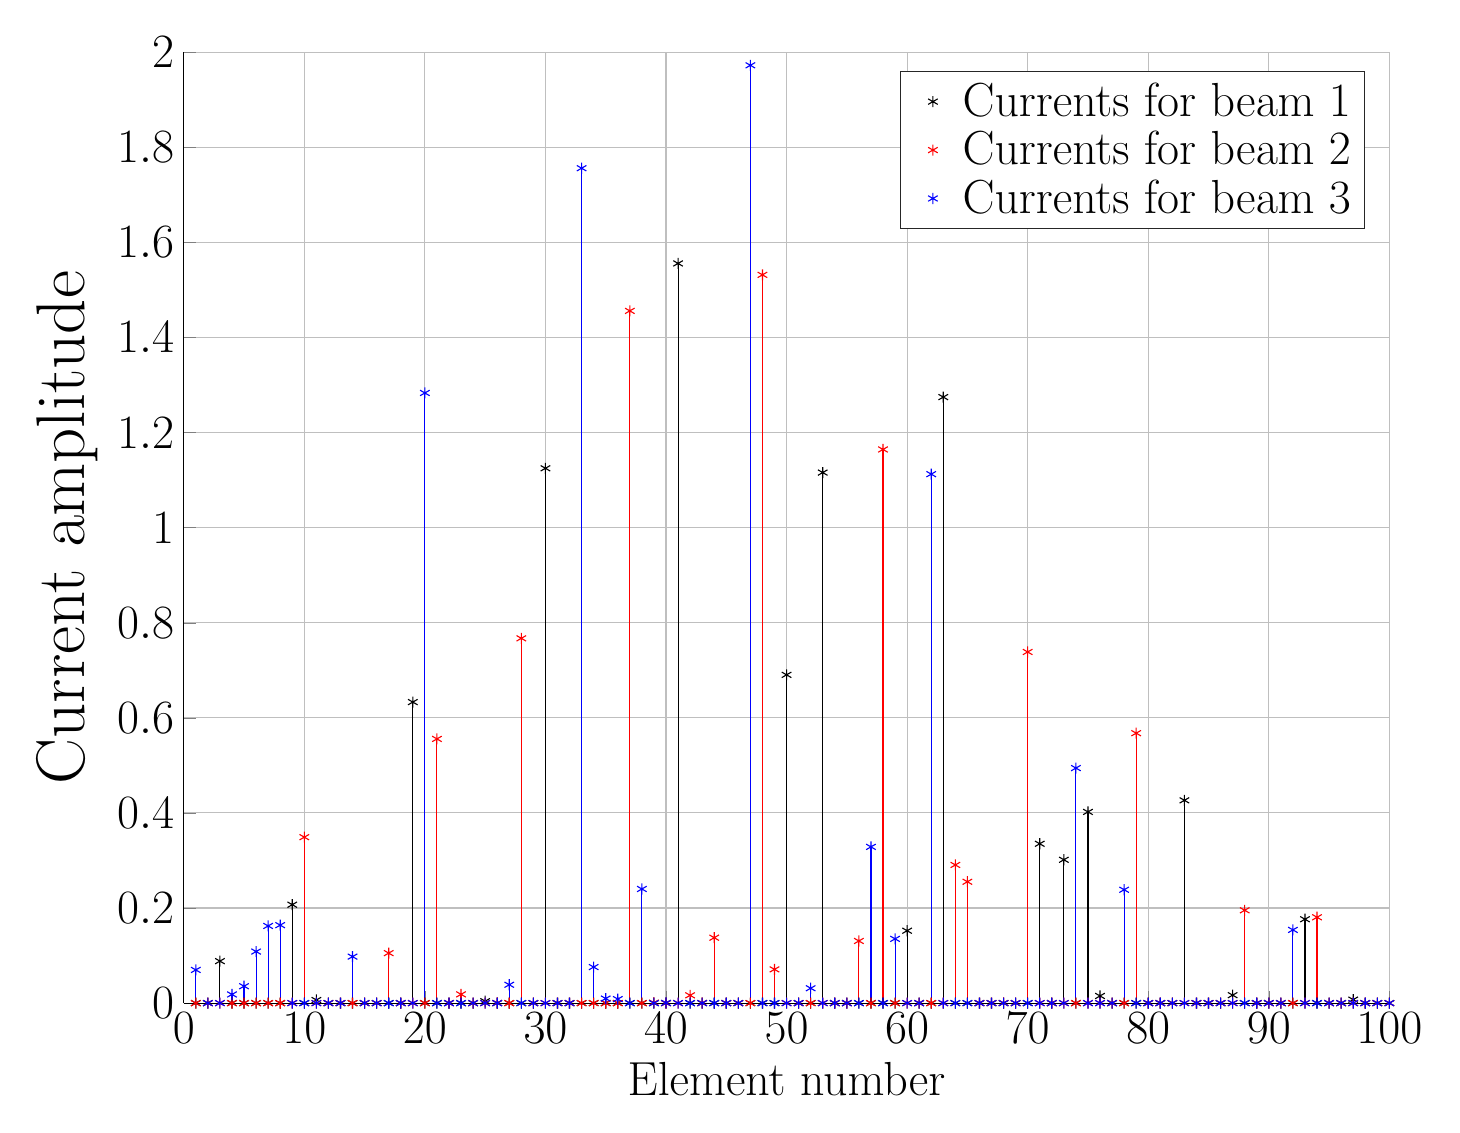
\begin{tikzpicture}

\begin{axis}[%
width=6.028in,
height=4.754in,
at={(1.011in,0.642in)},
scale only axis,
xmin=0,
xmax=100,
xlabel={Element number},
xmajorgrids,
ymin=0,
ymax=2,
ylabel={Current amplitude},
ymajorgrids,
axis background/.style={fill=white},
axis x line*=bottom,
axis y line*=left,
legend style={legend cell align=left,align=left,draw=white!15!black},
xlabel style={font=\LARGE},ylabel style={font=\Huge},legend style={font=\LARGE},ticklabel style={font=\LARGE}
]
\addplot[ycomb,color=black,solid,mark=asterisk,mark options={solid}] plot table[row sep=crcr] {%
1	0\\
2	0\\
3	0.0882955116063392\\
4	1.82387733129509e-288\\
5	0\\
6	0\\
7	0\\
8	0\\
9	0.206994904248721\\
10	0\\
11	0.00650668199739337\\
12	3.17619228925984e-229\\
13	0\\
14	0\\
15	0\\
16	6.55551983505469e-10\\
17	0\\
18	8.94296552522097e-05\\
19	0.633187367355409\\
20	0\\
21	0\\
22	0\\
23	0\\
24	0\\
25	0.00401604691046763\\
26	1.41668264345757e-245\\
27	0\\
28	0\\
29	0\\
30	1.12496093405858\\
31	0\\
32	0\\
33	0\\
34	3.38027611487321e-48\\
35	0\\
36	0\\
37	0\\
38	0\\
39	0\\
40	0\\
41	1.55586997192618\\
42	0\\
43	0\\
44	0\\
45	3.79339723806099e-97\\
46	7.87968202747556e-25\\
47	0\\
48	0\\
49	0\\
50	0.690501085515732\\
51	0\\
52	0\\
53	1.11596536750381\\
54	0\\
55	0\\
56	0\\
57	0\\
58	0\\
59	0\\
60	0.152251775463774\\
61	8.07579851351801e-63\\
62	0\\
63	1.27474127662515\\
64	0\\
65	0\\
66	0\\
67	0\\
68	0\\
69	4.94065645841247e-324\\
70	0\\
71	0.335158098580192\\
72	0\\
73	0.301490026448818\\
74	0\\
75	0.402161918846244\\
76	0.0150202540627461\\
77	0\\
78	0\\
79	2.17067462465211e-246\\
80	2.01870349064891e-22\\
81	0\\
82	0\\
83	0.426509478408387\\
84	0\\
85	0\\
86	0\\
87	0.0167085796152589\\
88	0\\
89	0\\
90	0\\
91	3.45019023231001e-58\\
92	0\\
93	0.17638480863685\\
94	0\\
95	5.5895047601318e-68\\
96	1.20473110519207e-64\\
97	0.00729888159840812\\
98	0\\
99	0\\
100	9.3859723977077e-172\\
};
\addlegendentry{Currents for beam 1};

\addplot[ycomb,color=red,solid,mark=asterisk,mark options={solid}] plot table[row sep=crcr] {%
1	0\\
2	0\\
3	0\\
4	0\\
5	0\\
6	0\\
7	0\\
8	0\\
9	0\\
10	0.34902058172907\\
11	0\\
12	0\\
13	0\\
14	0\\
15	0\\
16	0\\
17	0.105123288752876\\
18	0\\
19	0\\
20	0\\
21	0.555675863162067\\
22	0\\
23	0.01839108311685\\
24	0\\
25	0\\
26	0.000280330650380855\\
27	0\\
28	0.767285206820543\\
29	0\\
30	0\\
31	0\\
32	0\\
33	0\\
34	0\\
35	0\\
36	0\\
37	1.45604546824628\\
38	4.0431475252495e-220\\
39	0.000850069545760301\\
40	0\\
41	0\\
42	0.0163581904620457\\
43	0.000226851391132208\\
44	0.137551509401625\\
45	0\\
46	0\\
47	0\\
48	1.5318793291763\\
49	0.0709383824577087\\
50	0\\
51	0\\
52	0\\
53	0\\
54	0\\
55	4.79262641956573e-220\\
56	0.130689270214991\\
57	0\\
58	1.16457271755406\\
59	0\\
60	0\\
61	0\\
62	4.74162727616895e-246\\
63	0\\
64	0.290607591701805\\
65	0.255257192994946\\
66	0\\
67	5.0241619522281e-11\\
68	0.000226751853472731\\
69	0\\
70	0.738579727965347\\
71	0\\
72	0\\
73	0\\
74	0\\
75	0\\
76	0\\
77	0\\
78	0\\
79	0.567783976225254\\
80	0\\
81	0\\
82	0\\
83	0\\
84	4.21084270358136e-176\\
85	3.38093080128764e-86\\
86	1.04734816150376e-122\\
87	0\\
88	0.195220379898682\\
89	3.32502779702932e-11\\
90	0\\
91	0\\
92	0\\
93	0\\
94	0.180528824045936\\
95	0\\
96	0\\
97	0\\
98	0\\
99	0\\
100	0\\
};
\addlegendentry{Currents for beam 2};

\addplot[ycomb,color=blue,solid,mark=asterisk,mark options={solid}] plot table[row sep=crcr] {%
1	0.0697816025707138\\
2	7.59309176738369e-283\\
3	0\\
4	0.0182030115653807\\
5	0.0355052116186164\\
6	0.108459949535809\\
7	0.162277853432601\\
8	0.163983293686418\\
9	0\\
10	0\\
11	0\\
12	8.27023407818076e-17\\
13	0\\
14	0.0977820656446664\\
15	2.45783130219966e-24\\
16	0\\
17	0\\
18	0\\
19	0\\
20	1.28341677980869\\
21	0\\
22	1.28972828046307e-08\\
23	0\\
24	6.82505837240215e-09\\
25	2.9367783821872e-228\\
26	0\\
27	0.0386056916853912\\
28	0\\
29	0\\
30	0\\
31	0\\
32	7.13578626043079e-28\\
33	1.75616392651842\\
34	0.07579910491731\\
35	0.00956825452905467\\
36	0.00838067353634931\\
37	0\\
38	0.240044648011493\\
39	5.41173969046975e-95\\
40	0.000374832320732243\\
41	0\\
42	0\\
43	0\\
44	0\\
45	0\\
46	0\\
47	1.97261325635197\\
48	0\\
49	0\\
50	0\\
51	0\\
52	0.031258106642056\\
53	0\\
54	0\\
55	0\\
56	0\\
57	0.328609482022235\\
58	0\\
59	0.135134688261724\\
60	0\\
61	0\\
62	1.11264752365393\\
63	0\\
64	0\\
65	0\\
66	0\\
67	0\\
68	0\\
69	0\\
70	0\\
71	0\\
72	0\\
73	0\\
74	0.494385146857527\\
75	0\\
76	0\\
77	0\\
78	0.238426091797012\\
79	0\\
80	0\\
81	0\\
82	0\\
83	0\\
84	0\\
85	0\\
86	0\\
87	0\\
88	0\\
89	0\\
90	0\\
91	0\\
92	0.153988118765982\\
93	0\\
94	0\\
95	1.22636265067595e-26\\
96	0\\
97	7.48175851550487e-175\\
98	1.09596156712378e-59\\
99	0\\
100	0\\
};
\addlegendentry{Currents for beam 3};

\end{axis}
\end{tikzpicture}%
            \end{adjustbox}
        \end{column}
\end{columns}   

\end{frame}



\begin{frame}[t]{Beam-forming procedure}
 
\textbf{Two steps}:
\begin{itemize}
    \item Perform frequency allocation.
    \item Run optimal beam-forming algorithm.
\end{itemize}



\end{frame}


%
% -----------------------------------------------------------------------------------------------------------------
%



\end{document}

